\begin{defproblem}{diferencialny-pocet-279}
Výpočtom $\lim_{x \rightarrow a}\frac{f(x)-f(a)}{x-a}$ nájdite deriváciu funkcie $f$ v bode $a$, ak:
\begin{tasks}(2)
    \task $f(x)=x^2,a=0,1$
    \task $f(x)=2\cdot \sin 3x,a=\frac{\pi}{6}$
    \task $f(x)=1+2\cdot \ln x,a=1$
    \task $f(x)=\arcsin x,a=0$
    \task $f(x)=e^x,a=\ln 2$
\end{tasks}
\end{defproblem}

\begin{defproblem}{diferencialny-pocet-280}
Ukážte, že funkcia $f$ má v bode $a$ nevlastnú deriváciu, ak:
\begin{tasks}(2)
  \task $f(x)=\sqrt[3]{x-1},a=1$
  \task $f(x)=\sgn x,a=0$
\end{tasks}
\end{defproblem}

\begin{defproblem}{diferencialny-pocet-281}
Výpočtom $\lim\limits_{h \rightarrow 0}\frac{f(x+h)-f)(x)}{h}$ nájdite $f'(x)$ a
zistite definičný obor funkcie $f'$, ak:
\begin{tasks}(3)
    \task $f(x)=x^3+2x$
    \task $f(x)=x\cdot \sqrt[3]{x}$
    \task $f(x)=\frac{1}{1+x^2}$
    \task $f(x)=2^{x+1}$
    \task $f(x)=\ln x$
    \task $f(x)=\cot x+2$
    \task $f(x)=(x+1)^{\frac{2}{3}}$
    \task $f(x)=\sgn x$
\end{tasks}
\end{defproblem}

\begin{defproblem}{diferencialny-pocet-282}
Výpočtom príslušných limít nájdite $f'_+(a),f'_-(a)$, ak:
\begin{tasks}(2)
  \task $f(x)=|\cos x|; a=\frac{\pi}{2}$
  \task $f(x)=[x]\cdot \sin \pi x; a=1$
  \task! $f(x)=|x^2-5x+6|; a=2,a=3$
\end{tasks}
\end{defproblem}

\begin{defproblem}{diferencialny-pocet-283}
Porovnaním hodnôt $f'_+(a)$ a $f'_-(a)$ zistite, či existuje $f'(a)$, ak:
\begin{tasks}(2)
\task! $f(x) =
    \begin{cases}
      x, & $ak $ x<0 \\
      \ln (1+x), &  $ak $ x\geq 0
    \end{cases}
    $; $a=0$
\task! $f(x) =
    \begin{cases}
      x^2-1, & $ak $ x\leq -1 \\
      -2x, & $ak $ x>-1
    \end{cases}
    $; $a=-1$
\task $f(x)=x\cdot |x| ; a=0$
\task $f(x)=|\sin^3 x| ; a=\pi$
\end{tasks}
\end{defproblem}

\begin{defproblem}{diferencialny-pocet-284}
\begin{tasks}
\task
  Ak existuje vlastná derivácia funkcie $f$ v bode $0$, tak platí
  \[
    f'(0)=\lim_{h \rightarrow 0}\frac{f(h)-f(-h)}{2h}
  \]
  Dokážte!
\task
  Rozhodnite, či z existencie $\lim\limits_{h \rightarrow
  0}\frac{f(h)-f(-h)}{2h}$ vyplýva existencia $f'(0)$; svoje tvrdenie dokážte!
\end{tasks}
\end{defproblem}

\begin{defproblem}{diferencialny-pocet-285}
Ak $f':\mathbb{R}\rightarrow\mathbb{R}$ je derivácia nepárnej funkcie $f$, tak
$f'$ je párna funkcia. Dokážte! (Definíciu párnej a nepárnej funkcie pozri v
príklade $146.$)
\end{defproblem}

\begin{defproblem}{diferencialny-pocet-286}
Nájdite derivácie nasledujúcich funkcií:
\begin{tasks}(2)
  \task $y=2+x-x^2$
  \task $y=\frac{1+x-x^2}{1-x+x^2}$
  \task $y=\frac{3}{5}\cdot x^{\frac{5}{3}}-x^{-\sqrt{5}}$
  \task $y=\frac{\sqrt{x}}{2+\sqrt[3]{x^2}}$
  \task $y=(3x-7)^{10}$
  \task $y=x\cdot \sqrt{1+x^2}$
  \task $y=\frac{(1-x)^p}{(1+x)^q},p>1,q>0$
  \task $y=\frac{1}{\sqrt{1+x^2}\cdot (x+\sqrt{1+x^2})}$
  \task $y=\sqrt[13]{9+7\cdot \sqrt[5]{2x}}$
  \task $y=\sqrt{x+\sqrt{x+\sqrt{x}}}$
\end{tasks}
\end{defproblem}

\begin{defproblem}{diferencialny-pocet-287}
Nájdite $f'(a)$, ak
\[
  f(x)=(x-a)\varphi(x)
\]
kde $\varphi:\mathbb{R}\rightarrow\mathbb{R}$ je funkcia spojitá v bode $a$.
\end{defproblem}

\begin{defproblem}{diferencialny-pocet-288}
\begin{tasks}
\task
  Ukážte, že funkcia $f(x)=|x-a|\varphi(x)$, kde
  $\varphi:\mathbb{R}\rightarrow\mathbb{R}$ je spojitá funkcia a $\varphi(a)
  \neq 0$, nemá deriváciu v bode $a$.
\task
  Ukážte, že funkcia $f(x)=|x-a|^{1+\varepsilon}\varphi(x)$, kde
  $\varphi:\mathbb{R}\rightarrow\mathbb{R}$  je ohraničená na $\mathbb{R}$ a
  $\varepsilon>0$, má v bode $a$ deriváciu $f'(a)=0$.
\end{tasks}
\end{defproblem}

\begin{defproblem}{diferencialny-pocet-289}
Nájdite deriváciu funkcie
\begin{tasks}(2)
    \task $y=x\cdot\cos x$
    \task $y=\frac{\sin x-x\cdot\cos x}{\cos x+x\cdot\sin x}$
    \task $y=\frac{\sqrt{x}}{\tan x}$
    \task $y=\sin^n x\cdot\cos nx$
    \task $y=\sin (\cos^2 x)\cdot \cos (\sin^2 x)$
    \task $y=\frac{\sin^2 x}{\sin x^2}$
    \task $y=\frac{\sin^2 x}{1+\cot x}+\frac{\cos^2 x}{1+\tan x}$
    \task $y=\sqrt{1+\tan (x^2+x^{-2})}$
\end{tasks}
\end{defproblem}

\begin{defproblem}{diferencialny-pocet-290}
Nájdite derivácie funkcií:
\begin{tasks}(2)
  \task $y = (\sqrt{2})^x+(\sqrt{5})^{-x}$
  \task $y = e^{-x^2}$
  \task $y = e^x(x^2-2x+2)$
  \task $y = 2^{\sin x^2}$
  \task $y = e^{\sqrt{\frac{1-x}{1+x}}}$
  \task $y = e^{ax} \cdot \frac{a \cdot \sin{bx} - b \cdot \cos{bx}}{\sqrt{a^2+b^2}}$
  \task $y = (\frac{a}{b})^x \cdot (\frac{b}{x})^a \cdot (\frac{x}{a})^b$
  \task! $y = (\frac{1-x^2}{2} \sin{x} - \frac{(1+x)^2}{2} \cos{x}) \cdot e^{-x}$
\end{tasks}
\end{defproblem}

\begin{defproblem}{diferencialny-pocet-291}
Možno tvrdiť, že neexistuje $(f+g)'(a)$ (funkcie $f,g$ sú definované v okolé
bodu $a$),ak:
\begin{tasks}
\task existuje vlastná $f'(a)$ a neexistuje $g'(a)$?
\task $f$ má v bode $a$ nevlastnú deriváciu a neexistuje $g'(a)$?
\task neexistuje $f'(a)$ ani $g'(a)$?
\end{tasks}
\end{defproblem}

\begin{defproblem}{diferencialny-pocet-292}
Nech $f,g$ sú spojité funkcie definované na $\mathbb{R}$
\begin{align*}
  f'(g(a)) > 0 && g'(a) = +\infty
\end{align*}
Potom existuje nevlastná derivácia funkcie $f \circ g$ v bode $a$. Dokážte!
\end{defproblem}

\begin{defproblem}{diferencialny-pocet-293}
Nájdite derivácie funkcií:
\begin{tasks}(2)
    \task $y=\log_{3}(\tan \frac{x}{2})$
    \task $y=\frac{1}{4}\ln \frac{x^2-1}{x^2+1}$
    \task $y=\ln (x+\sqrt{x^2+1})$
    \task $y=e^{\sqrt{\log_2(x^2+x+1)}}$
    \task! $y=x\cdot\ln (x+\sqrt{1+x^2})-\sqrt{1+x^2}$
    \task! $y=\frac{1}{2} \ln (1+x)-\frac{1}{4} \ln (1+x^2)-\frac{1}{2\cdot(1+x)}$
    \task! $y=\frac{1}{\sin a}\cdot\ln \frac{1+x}{1-x}-\cot a\cdot\ln \frac{1+x\cdot\cos a}{1-x\cdot\cos a}$
    \task $y=x\cdot(\sin(\ln x)-\cos(\ln x))$
    \task! $y=\sqrt{x^2+1}-\ln (\frac{1}{x}+\sqrt{1+\frac{1}{x^2}})$
    \task $y=\log_2 x\cdot\log_3 x\cdot\ln x$
\end{tasks}
\end{defproblem}

\begin{defproblem}{diferencialny-pocet-294}
Nájdite derivácie funkcií:
\begin{tasks}(2)
    \task $y=\sqrt{x}-\arctan\sqrt{x}$
    \task $y=x\cdot\arcsin x$
    \task $y=\frac{\arccos x}{\arcsin xc}$
    \task $y=\arctan \frac{x}{1+\sqrt{1-x^2}}$
    \task $y=\ln (\arccos \frac{1}{\sqrt{x}})$
    \task $y=3^{\arctan(2x+\pi)}$
    \task $y=\arcsin(\frac{\sin a\cdot \sin x}{1-\cos a\cdot\cos x})$
    \task $y=\frac{1}{\sqrt{2}\arcsin(\sqrt{\frac{2}{3}}\sin x)}$
    \task! $y=x\cdot\arcsin \sqrt{\frac{x}{1+x}}+\arctan \sqrt{x}-\sqrt{x}$
    \task! $y=x\cdot(\arcsin x)^2+2\sqrt{1-x^2}\cdot\arcsin x-2x$
\end{tasks}
\end{defproblem}

\begin{defproblem}{diferencialny-pocet-295}
Nájdite derivácie funkcií:
\begin{tasks}(2)
    \task $y=\frac{1+x^2}{\sqrt[3]{x^4}\sin^7 x}$
    \task $y=\frac{\sqrt{x-1}}{\sqrt[3]{(x+2)^2}}\cdot\sqrt{(x+3)^3}$
    \task $y=\sqrt[3]{\frac{\sin 3x}{1-\sin 3x}},x\in(0,\frac{\pi}{6})$
    \task $y=x^x,x>0$
    \task $y=\sqrt[x]{x},x>0$
    \task $y=x^{x^2},x>0$
    \task! $y=(\cos x)^{\sin x}+(\sin x)^{\cos x},x\in(0,\frac{\pi}{2})$
\end{tasks}

\begin{solution}
  \textbf{a):}
  Výpočet sa zjednoduší nasledujúcou úvahou: ak funkcia $f$ má v bode $a$
  deriváciu a $f(a)\neq 0$, tak $(\ln |f|)'(a)=\frac{1}{f(a)}\cdot f'(a)$;
  odtiaľ možno vyjadriť $f'(a)=f(a)\cdot (\ln |f|)'(a)$. V našom prípade
  \[
    y=\frac{1+x^2}{\sqrt[3]{x^4}\cdot\sin^7 x}\cdot (\ln |y|)'
    = (\ln |1+x^2|-\frac{4}{3}\ln |x|-7\cdot\ln |\sin x|)' =
  \]
  \[
    = \frac{2x}{1+x^2}-\frac{4}{3x}-7\cdot \cot x
    = \frac{2x^2-4}{3x\cdot (1+x^2)}-7\cot x
  \]
  Teda
  \[
    y'=\frac{1+x^2}{\sqrt[3]{x^4}\cdot \sin^7 x}\cdot
    (\frac{2x^2-4}{3x\cdot (1+x^2)}-7\cdot\cot x)
  \]

  \textbf{d):}
  Funkcie tvaru $f^g$ (o funkcii $f$ predpokladáme, že je nezáporná) možno
  derivovať na základe úvahy z riešenia príkladu $295.(a)$ alebo (čo je vlastne
  to isté) prepísať ich predpis do podoby $e^{g\cdot\ln f}$ a takto zapísanú
  funkciu potom derivovať na základe viet o derivácii súčinu a zloženej funkcie.

  V našom prípade
  \[
    (x^x)'=(e^{x\cdot\ln x})'=e^{x\cdot\ln x}\cdot(x\cdot\ln x)'
    = x^x\cdot(\ln x +1)
  \]
\end{solution}
\end{defproblem}

\begin{defproblem}{diferencialny-pocet-296}
Uveďte príklad funkcií $f,g$ takých, že
\begin{tasks}
\task neexistujú $f'(a)$ ani $g'(a)$, ale existuje vlastná $(f\cdot g)(a)$
\task neexistuje $g'(a)$, ale existujú vlastné $f'(a)$ a $(f\cdot g)'(a)$
\end{tasks}
(Inšpiráciou môžu byť príklady $287.$ a $288$.)
\end{defproblem}

\begin{defproblem}{diferencialny-pocet-297}
Nech $f:\mathbb{R}\rightarrow\mathbb{R}$ je spojitá funkcia, nech v bode $a$ je
$f(a)\neq 0$ a existuje nevlastná $f'(a)$. Potom funkcia $\frac{1}{f}$ má v bode
$a$ nevlastnú deriváciu $-f'(a)$. Dokážte!
\end{defproblem}

\begin{defproblem}{diferencialny-pocet-298}
Nech funkcia $f$ je derivovaná v okolí $O(a)$ bodu $a$, pričom pre všetky $x\in
O(a)$ platí $|f(x)-f(a)|<K\cdot |x-a|$, kde $K$ je kladná konštanta. Nech
funkcia $g$ má deriváciu v bode $f(a),g'(f(a))=0$. Potom funkcia $g \circ f$ má
deriváciu v bode $a$ rovnú $0$. Dokážte!
\end{defproblem}

\begin{defproblem}{diferencialny-pocet-299}
Nájdite derivácie funkcií:
\begin{tasks}
\task $y=\ln \frac{b+a\cdot\cos x +\sqrt{b^2-a^2}\cdot \sin x}{a+b\cdot\cos x},x\in (0,\frac{\pi}{2}),0\leq a<b$
\task $y=\ln (1+\sin^2 x)-2\cdot\sin x \cdot \arctan(\sin x)$
\task $y=\frac{\arccos x}{x}+\frac{1}{2}\cdot \ln \frac{1-\sqrt{1-x^2}}{1+\sqrt{1-x^2}}$
\task $y=x\cdot\ln^2(x+\sqrt{1+x^2})-2\sqrt{1+x^2}\cdot\ln(x+\sqrt{1+x^2})+2x$
\task $\ln\frac{x+a}{\sqrt{x^2+b^2}}+\frac{a}{b}\arctan\frac{x}{b}$
\task $y=\frac{1}{4\sqrt{2}}\ln\frac{x^2+x\sqrt{2}+1}{x^2-x\sqrt{2}+1}-\frac{1}{2\sqrt{2}}\arctan\frac{x\sqrt{2}}{x^2-1}$
\task $y=x-\ln\sqrt{1+e^{2x}}+e^{-x}arccot e^{x}$
\task $y=\frac{3-\sin x}{2}\sqrt{\cos^2 x-2\sin x}+2\arcsin x\cdot\frac{1+\sin x}{\sqrt{2}}$
\task $y=e^{\arcsin x}(\cos (m\cdot\arcsin x)+\sin (m\arcsin x)),|x|<1$
\task $y=\ln\sqrt{x^2-2x\cdot\cos a +1}+\cot\cdot\arctan\frac{x-\cos a}{\sin a}$
\task $y=|(x-1)^2\cdot(x+1)^3|$
\task $y=[x]\cdot\sin^2 \pi x$
\task $y =
    \begin{cases}
      1-x & $, ak $ x<1 \\
      (1-x)(2-x) & $, ak $ x \in \interval{1}{2} \\
      -(2-x) &  $, ak $ x>2
    \end{cases}
    $
\task $y =
    \begin{cases}
    \arctan x & $, ak $ |x|\leq 1 \\
    \frac{\pi}{4}\sgn x+\frac{x-1}{2} &  $, ak $ |x|>1
    \end{cases}
    $
\task $y=\ln (ch x)+\frac{1}{2\cdot ch^2 x}$
\task $y=\frac{(\ln x)^x}{x^{\ln x}}$
\task $y=(\arcsin \sin^2 x)^{\arctan x}$
\task $y=x^{x^x}$
\task $y=x^{\frac{2}{\ln x}}-2x^{\log_x e}\cdot e^{1+\ln x}+e^{1+\frac{2}{\log_x e}}$
\end{tasks}
\end{defproblem}

\begin{defproblem}{diferencialny-pocet-300}
Ako treba vybrať koeficienty $a,b$, aby funkcia
\[
  f(x) =
    \begin{cases}
      x^2   & $, ak $ x \leq x_0 \\
      ax+b  &  $, ak $ x>x_0
    \end{cases}
\]
bola spojitá a mala deriváciu v každom bode $x\in\mathbb{R}$?
\end{defproblem}

\begin{defproblem}{diferencialny-pocet-301}
Ak funkcie $f_1,...,f_n$ majú deriváciu v bode $a$, tak
\begin{align*}
  (f_1 \cdot f_2 \cdot ... \cdot f_n)'(a)
  &= f'_1(a)\cdot f_2(a)\cdot ... \cdot f_n(a) + \\
  &+ f_1(a) \cdot f'_2(a) \cdot f_3(a) \cdot ... \cdot f_n(a) \\
  &+ ... \\
  &+ f_1(a) \cdot ... \cdot f_{n-1}(a) \cdot f'_n(a)
\end{align*}
Dokážte! Na základe toho nájdite $f'(0)$, ak
$f(x)=x\cdot(x-1)\cdot...\cdot (x-1000)$.
\end{defproblem}

\begin{defproblem}{diferencialny-pocet-302}
Nech nezáporné funkcie $f,g$ majú deriváciu v každom bode $x\in\mathbb{R}$.
Nájdite deriváciu funkcie $y$, ak
\begin{tasks}(2)
    \task $y=\sqrt{f^2(x)+g^2(x)}$
    \task $y=\arctan \frac{f(x)}{g(x)}$
    \task $y=\log_{f(x)}g(x)$ $(f(x)>1)$
    \task $y=f(x^2)$
    \task $y=f(\sin^2 x)+g(\cos^2 x)$
    \task $y=f(e^x)\cdot e^{f(x)}$
\end{tasks}
\end{defproblem}

\begin{defproblem}{diferencialny-pocet-303}
Nájdite vzorce pre súčty:
\begin{tasks}
\task $P_n(x)=1+2x+3x^2+...+nx^{n-1}$
\task $Q_n(x)=1+3x^2+5x^4+...+(2n-1)x^{2n-2},|x|\neq 1$
\task $R_n(x)=1^2+2^2x+3^2x^2+...+n^2x^{n-1},x\neq 1$
\task $T_n(x)=\cos x+2\cos 2x+...+n\cos nx,x\neq 2k\pi,(k\in\mathbb{Z})$
\end{tasks}
\end{defproblem}

\begin{defproblem}{diferencialny-pocet-304}
Ako treba voliť číslo $\alpha\in\mathbb{R}$ aby funkcia
$f(x) = \left\{ \begin{array}{r@{\quad}c}
    x^\alpha,& $ak $ x \neq 0 \\
    0, &  $ak $ x=0 \\ \end{array} \right.
    $
    bola
\begin{tasks}
    \task spojitá v bode $0$?
    \task mala deriváciu v bode $0$?
    \task mala deriváciu, ktorá je spojitá v bode $0$?
\end{tasks}
\end{defproblem}

\begin{defproblem}{diferencialny-pocet-305}
Možno použiť vetu o derivácii zloženej funkcie na výpočet derivácie funkcie
$y=\sin^2(\sqrt[3]{x^2})$ v bode $0$? Existuje táto derivácia?
\end{defproblem}

\begin{defproblem}{diferencialny-pocet-306}
Zostrojte funkciu $f:\mathbb{R}\rightarrow \mathbb{R}$ tak, aby
\begin{tasks}
\task
  definitným oborom jej derivácie bola množina $\{1,2\}$
\task
  bola rastúca, mala vlastnú alebo nevlastnú deriváciu v každom bode
  $x\in\mathbb{R}$ a pre každé $n\in\mathbb{Z}$ platilo $f'(n)=+\infty$
\task
  mala deriváciu v každom bode $x\in\mathbb{R}$, funkcia $f'$ bola nespokojná
  práve v bodoch množiny $\mathbb{N}\cup \{0\}$ a aby platilo $f'(n)=a$ ($a$ je
  dané reálne číslo) pre každé $n\in\mathbb{N}\cup \{0\}$
\end{tasks}
\end{defproblem}

\begin{defproblem}{diferencialny-pocet-307}
Nech funkcia $f$ má v bode $a$ obidve jednostranné derivácie. Potom $f$ je
spojitá v bode $a$. Dokážte!
\end{defproblem}

\begin{defproblem}{diferencialny-pocet-308}
Uveďte príklad funkcie, ktorá je spojitá v každom bode množiny $\mathbb{R}$ a
nemá vlastnú ani nevlastnú deriváciu v žiadnom bode množiny $\mathbb{N}$!
\end{defproblem}

\begin{defproblem}{diferencialny-pocet-309}
Uveďte príklad funkcie $f$ takej, že $f'(a)=-\infty$ a
\begin{tasks}
\task $f$ je spojitá v bode $a$
\task $a$ je bod nespojitosti $1.$ druhu funkcie $f$
\task $a$ je bod nespojitosti $2.$ druhu funkcie $f$
\end{tasks}
\end{defproblem}

\begin{defproblem}{diferencialny-pocet-310}
Nájdite deriváciu funkcie $f^{-1}$ v bode $b$, ak
\begin{tasks}
\task $f(x)=x+\frac{1}{5}x^5,\frac{\alpha}{b}=0,\frac{\beta}{b}=\frac{6}{5}$
\task $f(x)=2x-\frac{1}{2}\cos x,b=-\frac{1}{2}$
\task $f(x)=0,1x+e^{0,1x},b=1$
\task $f(x)=2x^2-x^4,x>1,b=0$
\task $f(x)=2x^2-x^4,x\in (0,1),b=\frac{3}{4}$
\end{tasks}

\begin{solution}
  \textbf{a):}
  Pretože $b=f(0)$ a $f'(x)=1+x^4$, je podľa vety $5$
  $(f^{-1})'(b)=\frac{1}{f'(0)}=1$. (Ako sa presvedčíme o rýdzomonotónnej
  funkcie $f$, ukážeme neskôr-pozri vetu $11.$)
\end{solution}
\end{defproblem}

\begin{defproblem}{diferencialny-pocet-311}
Odvoďte vzorec pre deriváciu inverznej funkcie z vety o derivácii zloženej
funkcie a stanovte predpoklady, za ktorých možno toto odvodenie vykonať!
\end{defproblem}

\begin{defproblem}{diferencialny-pocet-312}
Na základe vety o derivácii inverznej funkcie nájdite deriváciu funkcií
\begin{tasks}(3)
  \task $f(x)=\arcsin x$
  \task $f(x)=\arccos x$
  \task $f(x)=\arctan x$
  \task $f(x)=\arccot x$
  \task $f(x)=\ln x$
\end{tasks}
\end{defproblem}

\begin{defproblem}{diferencialny-pocet-313}
Nech $f$ je prostá funkcia definovaná na intervale
$\interval[open]{-\varepsilon}{\varepsilon}$, kde $\varepsilon$ je dané kladné
číslo, nech $f'(0)=\infty,f(0)=0$. Potom funkcia $f^{-1}$ má v bode $0$
deriváciu rovnú $0$. Dokážte!
\end{defproblem}

\begin{defproblem}{diferencialny-pocet-314}
Nájdite dotyčnicu v bode $A$ ku krivke $y=f(x)$, ak:
\begin{tasks}
\task
  $f(x)=(1+x)\sqrt[3]{3-x},\frac{\alpha}{A}=(-1,0),\frac{\beta}{A}=(2,3)$
\task
  $f(x)=|x-1|\ln (x+\sqrt{x^2+1}),A=(0,1)$
\task
  $f(x)=\sqrt[3]{x-1},A=(1,0)$
\task
  $f(x)=\frac{1}{1+x^2},A$ je priesečník krivky $y=f(x)$ s hyperbolou
  $y=\frac{1}{1+x}$
\end{tasks}
\end{defproblem}

\begin{defproblem}{diferencialny-pocet-315}
Nájdite rovnicu tej dotyčnice k parabole $y=x^2-2x+3$, ktorá je
\begin{tasks}
\task rovnobežná s priamkou $3x-y+5=0$
\task kolmá na priamku $x+y-1=0$
\end{tasks}
\end{defproblem}

\begin{defproblem}{diferencialny-pocet-316}
\begin{tasks}
\task
  Aký musí byť vzťah medzi koeficientami $a,b,c$, aby sa parabola $y=ax^2+bx+c$
  dotýkala priamky $y=0$?
\task
  Pre akú hodnotu parametra $a$ sa parabola $y=ax^2$ dotýka krivky $y=\ln x$?
\end{tasks}
\end{defproblem}

\begin{defproblem}{diferencialny-pocet-317}
Pomocou derivácie a diferenciálu nezávislej premennej zapíšte $df(a)$, ak
funkcia $f$ je daná predpisom:
\begin{tasks}(2)
  \task $f(x)=\frac{\ln x}{\sqrt{x}}$
  \task $f(x)=\sqrt{A^2+x^2}$
  \task $f(x)=\ln (1-x^2)$
  \task!
    $f(x)=\frac{\sin x}{2\cos^2 x}+\frac{1}{2}\ln |\tan (\frac{x}{2})
    + \frac{\pi}{4}|$
\end{tasks}
\end{defproblem}

\begin{defproblem}{diferencialny-pocet-318}
Nech $u,v,w$ sú kladné diferencovateľné funkcie, nájdite diferenciál funkcie $y$
v bode $a$, ak:
\begin{tasks}(3)
  \task $y=u\cdot v\cdot w$
  \task $y=\frac{u}{v^2}$
  \task $y=\arctan \frac{u}{w}$
  \task $y=\ln \sqrt{u^2+v^2}$
\end{tasks}
\end{defproblem}

\begin{defproblem}{diferencialny-pocet-319}
Pomocou diferenciálu odvoďte približné vzťahy pre výpočet nasledujúcich výrazov:
\begin{tasks}
\task $\sqrt{a^2+x^2},(a>0,x$ dostatočne malé)
\task $\ln (x+\sqrt{1+x^2})$ ($x$ blízke $0$)
\task $\arctan (1+x)$ ($x$ blízke $0$)
\task $\sqrt[n]{a^n+x}$ ($a>0$,$x$ blízke $0$)
\task $\ln (\tan \frac{x}{2})$ ($x$ blízke číslu $\frac{\pi}{2}$)
\end{tasks}

\begin{solution}
  \textbf{e):}
  Funkcia daná predpisom $f(x)=\ln (\tan \frac{x}{2})$ má v bode $\frac{\pi}{2}$
  deriváciu $f'(\frac{\pi}{2})=1$, preto je podľa vety $6$ diferencovateľná a
  možno ju teda písať v tvare
  \[
    f(x)=f(\frac{\pi}{2})+f'(\frac{\pi}{2})\cdot
    (x-\frac{\pi}{2})+\omega(x)=(x-\frac{\pi}{2})+\omega(x)
  \]
  kde $\lim\limits_{x \rightarrow
  \frac{\pi}{2}}\frac{\omega(x)}{x-\frac{\pi}{2}}=0$. Zanedbaním funkcie
  $\omega(x)$ dostaneme približný vzorec $\ln (\tan \frac{x}{2})\approx
  (x-\frac{\pi}{2})$ pre $x$ blízke číslu $\frac{\pi}{2}$. (Geometricky to
  znamená, že hodnoty funkcie $f$ nahrádzame funkčnými hodnotami jej dotyčnice v
  bode $(\frac{\pi}{2},0)$, $\omega(x)$ vyjadruje chybu, ktorej sa pri takomto
  nahradení dopúšťame.)
\end{solution}
\end{defproblem}

\begin{defproblem}{diferencialny-pocet-320}
Nech funkcia $f$ je definovaná v okolí bodu $a\in\mathbb{R}$. Potom sú
nasledujúce dva výroky ekvivalentné:
\begin{tasks}
\task
  funkcia $f$ je diferencovateľná v bode $a$
\task
  existuje funkcia $\varphi$ (s rovnakým definičným oborom ako $f$), ktorá je
  spojitá v bode $a$, pričom platí $f(x)=f(a)+\varphi(x)(x-a)$
  (Výrok $(b)$ sa nazýva Čechova definícia diferenciálu.)
\end{tasks}
\end{defproblem}

\begin{defproblem}{diferencialny-pocet-321}
Nájdite $y''$, ak
\begin{tasks}(2)
  \task $y=x\cdot \sqrt{1+x^2}$
  \task $y=\frac{x}{\sqrt{1-x^2}}$
  \task $y=e^{-x^2}$
  \task $y=(1+x^2)\cdot \arctan x$
  \task $y=x\cdot \ln x$
  \task $y=x\cdot(\sin \ln x+\cos \ln x)$
\end{tasks}
\end{defproblem}

\begin{defproblem}{diferencialny-pocet-322}
Nájdite určené derivácie nasledujúcich funkcií:
\begin{tasks}(2)
\task! $y^{(6)},y^{(7)}; y=x\cdot (2x-1)^2(x+3)^3$
\task! $y^{(5)},y^{(6)}; y=(2x-7)^2(x+7)^3$
\task! $y^{(10)}; y=\sin x\cdot \sin 2x \cdot \sin 3x$
\task $y^{(10)}; y=\sqrt{x}$
\task $y^{(22)}; y=\frac{1-x}{1+x}$
\task $y^{(13)}; y=\frac{2x+1}{x^2+x-2}$
\task $y^{(15)}; y=\sin 2x\cdot\cos 4x$
\end{tasks}

\begin{solution}
  \textbf{a):}
  Funkcia $y$ je polynóm $6.$ stupňa, teda $y=a_0x^6+a_1x^5+...+a_6$ nie je
  ťažké vypočítať, že $a_0=4$. Potom
  \begin{align*}
    y^{VI}
    &= (a_0x^6+a_1x^5+...+a_6)^{VI} \\
    &= a_0(x^6)^{VI}+a_1(x^5)^{VI}+...+a_5x^{VI} \\
    &=6! \cdot a_0=6 \cdot 4=2880
  \end{align*}
  $y^{VII}=0$ (rád derivácie je vyšší ako stupeň polynómu).

  \textbf{e):}
  Funkciu $y$ možno zapísať v podobe, ktorá je pre derivovanie výhodnejšia:
  \begin{align*}
    y &= \frac{2x+1}{x^2+x-2}=\frac{2x+1}{(x+2)(x-1)} = \\
    &= \frac{(x+2)+(x-1)}{(x+2)(x-1)}=\frac{1}{x-1}+\frac{1}{x+2}
  \end{align*}
  Potom
  \begin{align*}
    y^{(13)}
      &=((x-1)^{-1})^{(13)}+((x+2)^{-1})^{(13)} = \\
    &=(-1)^{13}\cdot 13!(x-1)^{-14}+(-1)^{13}13!(x+2)^{-14} \\
    &=-(13!)(\frac{1}{(x-1)^{14}}+\frac{1}{(x+2)^{14}})
  \end{align*}

\end{solution}
\end{defproblem}

\begin{defproblem}{diferencialny-pocet-323}
Pomocou Leibnitzovho vzorca nájdite určené derivácie nasledujúcich funkcií:
\begin{tasks}(2)
\task $y^{(100)}; y=\frac{1+x}{\sqrt{1-x}}$
\task $y^{(5)}; y=x\cdot\ln x$
\task $y^{(50)}; y=x^2\sin 2x$
\task $y'''; y=y=\frac{\cos 3x}{\sqrt[3]{1-3x}}$
\task $y^{(101)}; y=(x^2-2x)\cos 3x$
\task $y^{(16)}; y=(x-\sin x)^2$
\task $y^{(100)}; y=x\cdot\sin x\cdot\cos 2x$
\end{tasks}
\end{defproblem}

\begin{defproblem}{diferencialny-pocet-324}
AK funkcia $f$ má derivácie až do rádu $n$, tak platí
\[
  (f(ax+b))^{(n)}=a^nf^{(n)}(ax+b)
\]
Dokážte!
\end{defproblem}

\begin{defproblem}{diferencialny-pocet-325}
Nájdite $y^{(n)}$, ak:
\begin{tasks}(3)
  \task $y=\ln (ax+b)$
  \task $y=\frac{1}{x\cdot(1-x)}$
  \task $y=\frac{1}{x^2-3x+2}$
  \task $y=\frac{1}{\sqrt{1-2x}}$
  \task $y=\sin^2 x$
  \task $y=\sin3x \cdot \cos 5x$
  \task $y=\sin^4 x+\cos^4 x$
  \task $y=\sin^2 ax \cdot \cos bx$
\end{tasks}
\end{defproblem}

\begin{defproblem}{diferencialny-pocet-326}
Nájdite $y^{(n)}$, ak:
\begin{tasks}(2)
  \task $y=(x-1)\cdot 2^{x-1}$
  \task $y=\frac{x}{\sqrt[3]{1+x}}$
  \task $y=x^2\sin bx$
  \task $y=(x^2+2x+2)\cdot e^{-x}$
  \task $y=x\cdot\log_{2}(1-3x)$
  \task $y=(3-2x)^2\cdot e^{2-3x}$
\end{tasks}
\end{defproblem}

\begin{defproblem}{diferencialny-pocet-327}
Nájdite $f^{(n)}(0)$, ak:
\begin{tasks}(3)
  \task $y=\frac{1}{(1-2x)(1+x)}$
  \task $y=x^2e^{2x}$
  \task $y=\frac{x}{\sqrt{1-x}}$
  \task $y=\frac{x}{1-x^2}$
  \task $y=\arcsin x$
  \task $y=\arctan x$
  \task $y=\frac{1}{(1-x^2)^2}$
\end{tasks}

\begin{solution}
  \textbf{f):}
  Pretože $f'(x)=\frac{1}{1+x^2}$, platí $(1+x^2)f'(x)=1$ pre všetky $x
  \in\mathbb{R}$. To znamená, že funkcia $(1+x^2)f'(x)$ je na $\mathbb{R}$
  konštantná, preto jej derivácie všetkých rádov sú rovné $0$:
  \[
    [(1+x^2)f'(x)]^{(k)}=0,(k\in\mathbb{N})
  \]
  Položme $k=n-1$; pre $n=2$ má uvedená rovnosť tvar $(*)$
  \[
    (1+x^2)f''(x)+2x\cdot f'(x)=0
  \]
  a pre $n\geq 3$ použitím Leibnitzovho vzorca dostaneme
  \[
    (1+x^2)f^{(n)}(x)+2(n-1)x\cdot f^{(n-1)}(x)+(n-1)(n-2)f^{(n-2)}(x)=0
  \]
  (Až pre $k \geq 2$,t.j. $n\geq 3$, obsahuje Leibnitzov vzorec všetky nenulové
  derivácie funkcie $1+x^2$, zápis prvej derivácie funkcie $(1+x^2)f'(x)$ sa
  teda odlišuje od zápisu k-tej derivácie tejto funkcie pre $k\geq 2$, preto
  treba prípad $k=1$ robiť samostatne.)

  Ak v poslednej rovnosti položíme $x=0$, dostávame pre $n\geq 3$
  \[
    f^{(n)}(0)=-(n-1)(n-2)f^{(n-2)}(0)
  \]
  čo je rekurentný vzťah pre vyjadrenie $f^{(n)}(0)$. Dosadením do predpisu pre
  $f'$ dostaneme $f'(0)=1$, z $(*)$ vychádza $f''(0)=0$. Na základe toho môžeme
  matematickou indukciou dokázať, že
  \[
    f^{(2k+2)}(0)=0,f^{(2k+1)}(0)=(-1)^k(2k) ; k=0,1,2,...
  \]

  \textit{Poznámka:}
  Prechádzajúca úvaha má (našťastie len zdanlivo) jeden nedostatok: ak chceme
  použiť Leibnitzov vzorec na výpočet $(n-1)$-vej derivácie súčinu $(1+x^2)\cdot
  f'(x)$, treba sa najprv presvedčiť, že existujú $(n-1)$-vé derivácie funkcií
  $(1+x^2)$ a $f'(x)$ (t.j. $(1+x^2)^{(n-1)}$ a $f^{(n)}(x)$); to sme ale
  neurobili.

  Dokázať, že existuje $(1+x^2)^{(n-1)}$, je ľahké; zostávateda dokázať
  existenciu $(\arctan x)^{(n)}$. (Návod: možno postupovať indrukciou; z
  predpokladu, že $f^{(k-1)}$ je podielom polynómov $P_{k-1}$ a $Q_{k-1}$ nemá
  reálne korene, vyplýva na základe vety o derivácii podielu, že $f^{(k)}$
  existuje a možno ju zapísať v tvare podielu polynómov $P_k$ a $Q_k$, pričom
  $Q_k$ nemá reálne korene.)
\end{solution}
\end{defproblem}

\begin{defproblem}{diferencialny-pocet-328}
Dokážte, že funkcia definovaná predpisom
\[
  f(x) =
  \begin{cases}
    x^{2n \sin \frac{1}{x}} & $, ak $ x \neq 0 \\
    0 &  $, ak $ x=0
  \end{cases}
\]
$n\in\mathbb{N}$ má v bode $0$ derivácie až do rádu $n$, ale nemá $(n+1)$-vú deriváciu v tomto bode.
\end{defproblem}

\begin{defproblem}{diferencialny-pocet-329}
Nech funkcia $f$ je spojitá na intervale $\interval[open]{a}{b}$, kde
$a<b,a,b\in\mathbb{R^*}$, nech pre každé $x\in \interval[open]{a}{b}$ existuje
vlastná alebo nevlastná nenulová $f'(x)$. Potom $f$ je prostá na intervale
$\interval[open]{a}{b}$. Dokážte!
\end{defproblem}

\begin{defproblem}{diferencialny-pocet-330}
Nech funkcia $f$ je $n$-krát diferencovateľná na intervale $\interval{a}{b}$ (to
znamená, že existujú $f^{(1)},...,f^{(n)}$ definované na intervale
$\interval{a}{b}$) a má tam nulové hodnoty v $n+1$ bodoch. Potom existuje také
$o\in \interval[open]{a}{b}$, že $f^{(n)}(c)=0$. Dokážte!
\end{defproblem}

\begin{defproblem}{diferencialny-pocet-331}
Ak sú všetky korene polynómu
\[
  P_n(x)=a_0x^n+...+a_n; (a_0,...,a_n\in\mathbb{R},a_0\neq 0)
\]
reálne, tak aj jeho derivácie $P'_n,...,P_n^{(n-1)}$ majú len reálne korene.

(Komplexné číslo $a$ sa nazýva $m$-násobný koreň polynómu $P_n$($n\geq
m,n,m\in\mathbb{N}$), ak možno $P_n$ písať v tvare $P_n(x)=(x-a)^mQ_{n-m}(x)$,
pričom číslo $a$ nie je koreňom polynómu $Q_{n-m}$. Základná veta algebry
hovorí, že súčet násobností navzájom rôznych komplexných koreňov polynómu sa
rovná jeho stupňu. Teda polynóm $P_n$ stupňa $n$ má všetky korene reálne práve
vtedy, keď súčet násobností jeho navzájom rôznych reálnych koreňov je $n$.)
\end{defproblem}

\begin{defproblem}{diferencialny-pocet-332}
Ukážte, že rovnica $x^3-3x^2+6x-1=0$ má len jeden koreň, pričom tento koreň je
prostý (prostými sa nazývajú jednonásobné korene polynómu).
\end{defproblem}

\begin{defproblem}{diferencialny-pocet-333}
Nech funkcia $f:\interval[open]{a}{b}\rightarrow\mathbb{R}$, kde
$a<b,a,b\in\mathbb{R^*}$, je spojitá, má vlastnú alebo nevlastnú deriváciu v
každom bode $x\in \interval[open]{a}{b}$ a nech $\lim\limits_{x\rightarrow
a}f(x)=\lim\limits_{x\rightarrow a}f(x)$. Potom existuje $c\in
\interval[open]{a}{b}$, v ktorom $f'(c)=0$. Dokážte!
\end{defproblem}

\begin{defproblem}{diferencialny-pocet-334}
Zostrojte funkciu $f$ definovanú na intervale $\interval{a}{b}$, pre ktorú
$f(a)=f(b)$, pre každé $x\in \interval[open]{a}{b}$ existuje vlastná $f'(x)$ a
pre všetky $x\in \interval[open]{a}{b}$ platí $f'(x)\neq 0$.
\end{defproblem}

\begin{defproblem}{diferencialny-pocet-335}
Funkcia $y=1-\sqrt[3]{x^2}$ nadobúda nulové hodnoty pre $a=-1,b=1$, ale napriek
tomu nemá v žiadnom bode intervalu $\interval[open]{-1}{1}$ nulovú deriváciu. Je
to v rozpore s tvrdením Rolleho vety?
\end{defproblem}

\begin{defproblem}{diferencialny-pocet-336}
\begin{tasks}
\task
  Nech funkcia $f$ je definovaná na intervale $I$, pričom v každom bode $x\in I$
  platí $f'(x)=0$. Potom funkcia $f$ je konštantná na intervale $I$. Dokážte!
\task
  Uveďte príklad takej funkcie definovanej na otvorenej množine $M$, že $f'=0$
  na $M$ a $f$ nie je konštantná na množine $M$!
\end{tasks}
\end{defproblem}

\begin{defproblem}{diferencialny-pocet-337}
Ukážte, že funkcie $f(x)=\arctan \frac{1+x}{1-x}$ a $g(x)=\arctan x$ majú
rovnaké derivácie v každom bode množiny $\interval[open]{-\infty}{1} \cup
\interval[open]{1}{\infty}$. Na základe toho odvoďte vzťah medzi funkciami $f$ a
$g$!

\begin{solution}
  Derivovaním dostaneme
  \begin{align*}
    f'(x) &= \frac{1}{1+x^2},x\in\mathbb{R}\setminus \{1\} \\
    g'(x) &= \frac{1}{1+x^2}
  \end{align*}
  Označme $h:=f-g$; potom $h'(x)=0$ pre $x\in \interval[open]{1}{\infty}$. Podľa
  výsledku príkladu $336$ je teda funkcia $h$ konštantná na intervale
  $\interval[open]{-\infty}{1}$ a konštantná na intervale
  $\interval[open]{1}{\infty}$. Hodnotu konštanty na intervale $(-\infty,1)$
  nájdeme ako funkčnú hodnotu v niektorom vhodne zvolenom bode, napr.
  \[
    k_1=h(0)=\arctan 1- \arctan 0=\frac{\pi}{4}
  \]
  Pretože výpočet $h(c)$ v niektorom $c\in \interval[open]{1}{\infty}$ by bol
  komplikovanejší, pomôžeme si nasledujúcou úvahou: pretože $h(x)=k_2$ na
  intervale $\interval[open]{1}{\infty}$, platí
  \[
    k_2=\lim_{x\rightarrow 1+}h(x)=-\frac{\pi}{2}-\frac{\pi}{4}=-\frac{3}{4}\pi
  \]
  Celkovo teda
  \[
    \arctan \frac{1+x}{1-x}-\arctan x =
    \begin{cases}
      \frac{\pi}{4}    & $,  ak $ x<1 \\
      -\frac{3}{4}\pi  & $, ak $ x>1
    \end{cases}
  \]
  čo môžeme prepísať do podoby
  \[
    \arctan \frac{1+x}{1-x}-\arctan x
    = -\frac{\pi}{2} \sgn (x-1)-\frac{\pi}{4},x \neq 1
  \]

\end{solution}
\end{defproblem}

\begin{defproblem}{diferencialny-pocet-338}
Dokážte rovnosti:
\begin{tasks}
\task $\arctan x=\frac{\pi}{2}-\arctan x,x \in \mathbb{R}$
\task $\arcsin x+\arccos x=\frac{\pi}{2},x \in \interval{-1}{1}$
\task $2\arctan x+\arcsin \frac{2x}{1+x^2}=\pi \sgn x,|x|\geq 1$
\task $3\arccos x-\arccos (3x-4x^3)=\pi ,|x|\leq \frac{1}{2}$
\task $\arcsin x=\arctan \frac{x}{\sqrt{1-x^2}},x\in \interval[open]{-1}{1}$
\end{tasks}
\end{defproblem}

\begin{defproblem}{diferencialny-pocet-339}
Nech funkcia $f$ je definovaná na intervale $I$, nech pre každé $x\in I$ platí
$f'(x)=k$ ($k$ je reálna konštanta). Potom $f(x)=kx+b$. Dokážte!
\end{defproblem}

\begin{defproblem}{diferencialny-pocet-340}
Dokážte, že funkcia $\sgn x$ nie je deriváciou žiadnej funkcia!
\end{defproblem}

\begin{defproblem}{diferencialny-pocet-341}
Dokážte nasledujúce nerovnosti:
\begin{tasks}
\task $|\sin x-\sin y|\leq |x-y|,x,y\in\mathbb{R}$
\task $p\cdot y^{p-1}(x-y)\leq x^p-y^p \leq p\cdot x^{p-1}(x-y)$, ak $0<y<x,p>1$
\task $|\arctan a-\arctan b|\leq |a-b|,a,b\in\mathbb{R}$
\task $\frac{a-b}{a}<\ln \frac{a}{b}<\frac{a-b}{b}$, ak $0<b<a$
\end{tasks}

\begin{solution}
  \textbf{a):}
  Pre $x=y$ Uvedená nerovnosť zrejme platí. Ak $x<y$ (dôkaz pre $x>y$ by bol
  rovnaký), tak na intervale $\interval{x}{y}$ funkcia $f(x)=\sin x$ vyhovuje
  predpokladom Lagrangeovej vety o strednej hodnote, podľa ktorej
  \[
    \sin x - \sin y = (x-y) \cos c
  \]
  pre niektoré $c\in \interval[open]{x}{y}$. Pretože $|\cos c|\leq 1$ pre
  ľubovoľné $c\in\mathbb{R}$, je
  \[
    |\sin x-\sin y|=|\cos c|\cdot|x-y|\leq |x-y|
  \]
\end{solution}
\end{defproblem}

\begin{defproblem}{diferencialny-pocet-342}
\begin{tasks}
\task
  Nech funkcia $f$ má na ohraničenom alebo neohraničenom intervale
  $\interval[open]{a}{b}$ ohraničenú deriváciu $f'$. Potom $f$ je rovnomerne
  spojitá na $\interval[open]{a}{b}$. Dokážte!
\task
  Ukážte, že funkcia $f(x)=x\cdot \sin \frac{1}{x}$ je rovnomerne spojitá na
  intervale $\interval[open]{0}{1}$, ale nemá tam ohraničenú deriváciu!
\end{tasks}
\end{defproblem}

\begin{defproblem}{diferencialny-pocet-343}
Nech funkcia $f$, ktorá má v každom bode ohraničeného intervalu
$\interval[open]{a}{b}$ deriváciu, nie je ohraničená na $\interval[open]{a}{b}$.
Potom funkcia $f'$ nie je ohraničená na $\interval[open]{a}{b}$. Dokážte!
\end{defproblem}

\begin{defproblem}{diferencialny-pocet-344}
Nech $f,F$ sú funkcie definované na otvorenom intervale $I \subset \mathbb{R},f$
je spojitá a pre každé $x,y\in I,x<y$, existuje $y\in (x,y)$ tak, že
$F(x)-F(y)=(x-y)\cdot f(z)$. Potom na intervale $I$ platí $F'=f$. Dokážte!
\end{defproblem}

\begin{defproblem}{diferencialny-pocet-345}
Nech derivácia funkcie $f$ je spojitá na uzavretom intervale $\interval{a}{b}$.
Možno tvrdiť, že pre každý bod $c\in \interval[open]{a}{b}$ existuje interval $\interval{
\alpha}{\beta} \subset \interval[open]{a}{b}$ taký, že $f'(c)\cdot
(\beta-\alpha)=f(\beta)-f(\alpha)$?
\end{defproblem}

\begin{defproblem}{diferencialny-pocet-346}
Nájdite chybu v nasledujúcom \enquote{dôkaze} Cauchyho vety:

Nech funkcie $f,g$ vyhovujú prvému, druhému a štvrtému predpokladu a nech
$g'(x)\neq 0$ pre $x\in \interval[open]{a}{b}$. Potom každá z funkcií $f,g$
vyhovuje predpokladom Lagrangeovej vety o strednej hodnote, a teda platí
$f(b)-f(a)=f'(c)(a-b),g(b)-g(a)=g'(c)(b-a)$ pre niektoré $c\in
\interval[open]{a}{b}$. Ak vydelíme prvú z týchto rovností druhou, dostaneme
\[\frac{f(b)-f(a)}{g(b)-g(a)}=\frac{f'(c)}{g'(c)}\]
\end{defproblem}

\begin{defproblem}{diferencialny-pocet-347}
Nech funkcia $f$ a jej derivácia sú definované na intervale $\interval{1}{2}$.
Potom existuje $c\in \interval[open]{1}{2}$ také, že
$f(2)-f(1)=\frac{c^2}{2}f'(c)$. Dokážte!
\end{defproblem}

\begin{defproblem}{diferencialny-pocet-348}
Nech funkcia $f$ a jej derivácia $f'$ sú definované na intervale
$\interval{a}{b}$, pričom $a\cdot b>0$. Dokážte, že potom existuje $c \in
\interval[open]{a}{b}$ také, že
\[
  \frac{1}{a-b}
  \begin{vmatrix}
    a & b \\
    f(a) & f(b)
  \end{vmatrix}
  =f(c)-cf'(c)
\]
\end{defproblem}

\begin{defproblem}{diferencialny-pocet-349}
Zistite, na ktorých intervaloch sú nasledujúce funkcie monotónne:
\begin{tasks}(3)
  \task $y=3x-x^3$
  \task $y=\frac{2x}{1+x^2}$
  \task $y=x+\sin x$
  \task $y=x+|\sin 2x|$
  \task $y=\cos \frac{\pi}{x}$
  \task $y=\frac{x^2}{2^x}$
  \task $y=x^2-\ln x^2$
  \task $y=
    \begin{cases}
      x(\sqrt{\frac{3}{2}}+\sin \ln x),& $ak $ x > 0 \\
      0, &  $ak $ x=0
    \end{cases}
    $
\end{tasks}
\end{defproblem}

\begin{defproblem}{diferencialny-pocet-350}
Nech funkcia $f: I \rightarrow\mathbb{R}$ Je rastúca na otvorenom intervale $I$
a diferencovateľná v každom bode $x\in I$. Potom $f'(x)\geq 0$ pre Každé $x\in
I$. Dokážte!
\end{defproblem}

\begin{defproblem}{diferencialny-pocet-351}
Pre každý polynóm $P_n$ stupňa $n\geq 1$ možno nájsť číslo $a>0$ tak, že $P_n$
je rýdzomonotónny na intervale $\interval[open]{-\infty}{-a}$ a rýdzomonotónny
na intervale $\interval[open]{a}{\infty}$. Dokážte!
\end{defproblem}

\begin{defproblem}{diferencialny-pocet-352}
Dokážte nasledujúce nerovnosti:
\begin{tasks}
\task $e^x>1+x$ pre $x\neq 0$
\task $x-\frac{x^3}{6}<\sin x<x$ pre $x>0$
\task $\tan x>x$ pre $0<x<\frac{\pi}{2}$
\task $\tan x>x+\frac{x^3}{3}$ pre $0<x<\frac{\pi}{2}$
\task $x^{\alpha}-1>\alpha\cdot(x-1)$ pre $\alpha\geq 2,x>1$
\task $\sqrt[n]{x}-\sqrt[n]{a}<\sqrt[n]{x-a}$ pre $n>1,x>a>0$
\task $1+2\cdot\ln x\leq x^2$ pre $x>0$
\end{tasks}
\end{defproblem}

\begin{defproblem}{diferencialny-pocet-353}
Dokážte nerovnosť $\frac{x}{1+x}<\ln (1+x)<x$ pre $x>-1$ a na jej základ
nerovnosť
\[
  \lim_{n \rightarrow \infty}(\frac{1}{n}+\frac{1}{n+1}+...+\frac{1}{2n})=\ln 2
\]
\end{defproblem}

\begin{defproblem}{diferencialny-pocet-354}
Nech $M$ je konečná podmnožina intervalu $I=\interval[open]{a}{b}$, kde $a<b, a,
b \in \mathbb{R^*}$, nech funkcia $f$ je spojitá na $I$ a má kladnú deriváciu v
každom bode $x\in I \setminus M$. Potom $f$ je rastúca na $I$. Dokážte!

(Všimnime si, že v predpokladoch tohto tvrdenia sa nehovorí nič o existencii
derivácie v bodoch množiny $M$; teda funkcia $f'$ môže byť definovaná v
niektorých (alebo aj vo všetkých) bodoch množiny $M$, ale pripúšťa sa aj
možnosť, že definičným oborom funkcie $f'$ je len množina $I \setminus M$.)
\end{defproblem}

\begin{defproblem}{diferencialny-pocet-355}
Nech funkcie $f,g$ sú diferencovateľné na intervale $\interval[open
right]{a}{\infty}, f(a)>g(a)$ a Nech pre všetky $x \in
\interval[open]{a}{\infty}$ platí $f'(x)\geq g'(x)$. Potom pre všetky $x\in
\interval[open right]{a}{\infty}$ platí $f(x)>g(x)$. Dokážte!
\end{defproblem}

\begin{defproblem}{diferencialny-pocet-356}
Musí byť derivácia monotónnej funkcie monotónna?
\end{defproblem}

\begin{defproblem}{diferencialny-pocet-357}
Zistite, na ktorých intervaloch sú nasledujúce funkcie rýdzo konvexné, resp.
rýdzo konkávne:
\begin{tasks}(3)
  \task $y=3x^2-x^3$
  \task $y=x+x^{\frac{5}{3}}$
  \task $y=x+\sin x$
  \task $y=\ln (1+x^2)$
  \task $y=x\cdot\sin (\ln x)$
  \task $y=\sqrt[3]{|x|}$
\end{tasks}
\end{defproblem}

\begin{defproblem}{diferencialny-pocet-358}
\begin{tasks}
\task
  Pre ktoré hodnoty $p\in\mathbb{N},q\in\mathbb{N}$ je bod $x=0$ inflexným bodom
  funkcie $y=x^{\frac{p}{q}}$ (predpokladáme, že $p,q$ sú nesúdeliteľné čísla)?
\task
  Akým podmienkam musia vyhovovať koeficienty $a\neq 0,b,c$, aby krivka
  $y=ax^4+bx^3+cx^2+dx+e$ mala inflexné body?
\task
  Pre aké hodnoty parametra $a$ je krivka $y=x^4+ax^3+\frac{3}{2}x^2+1$ konvexná
  na $\mathbb{R}$?
\end{tasks}
\end{defproblem}

\begin{defproblem}{diferencialny-pocet-359}
Nech funkcia $f$ je diferencovateľná v každom bode intervalu
$\interval[open]{a}{b}$, pričom $f'$ je na $\interval[open]{a}{b}$ rastúca.
Potom $f$ je rýdzo konvexná na $\interval[open]{a}{b}$. Dokážte!
\end{defproblem}

\begin{defproblem}{diferencialny-pocet-360}
Dokážte nasledujúce nerovnosti:
\begin{tasks}
\task $\frac{1}{2}(x^n+y^n)>(\frac{x+y}{2})^n$ pre $x>0,y>0,x\neq y,n>1$
\task $\frac{1}{2}(e^x+e^y)>e^{\frac{x+y}{2}}$ pre $x\neq y$
\task $x\cdot\ln x+\ln y>(x+y)\ln \frac{x+y}{2}$ pre $x>0,y>0,x\neq y$
\task $\frac{2}{\pi}x<\sin x$ pre $x\in (0,\frac{\pi}{2})$
\task $\arctan x+\arctan y>2\arctan \frac{x+y}{2}$ pre $x\neq y$
\task $x-1<\log_2 x$ pre $x\in (1,2)$
\end{tasks}

\begin{solution}
  \textbf{b):}
  Pretože $(e^x)''=e^x>0$ pre všetky $x\in\mathbb{R}$, je funkcia $f(x)=e^x$
  rýdzo konvexná na $\mathbb{R}$: teda platí
  \[
    \forall x,y\in \mathbb{R},x\neq y \forall p,q>0,p+q=1;f(px+qy)<pf(x)+qf(y)
  \]
  Ak špeciálne zvolíme $p=q=\frac{1}{2}$, dostaneme
  \[
    e^{\frac{x+y}{2}}
    = f(\frac{1}{2}x+\frac{1}{2}y)<\frac{1}{2}f(x)+\frac{1}{2}f(y)
    = \frac{1}{2}(e^x+e^y), x\neq y
  \]
\end{solution}
\end{defproblem}

\begin{defproblem}{diferencialny-pocet-361}
Ukážte, že neexistuje funkcia, ktorá je kladná na $\mathbb{R}$ a má v každom
bode $x\in\mathbb{R}$ zápornú druhú deriváciu.
\end{defproblem}

\begin{defproblem}{diferencialny-pocet-362}
\begin{tasks}
\task
  Nech $f$ je rýdzo konvexná a diferencovateľná na intervale $I$, nech $a\in I$.
  Potom na množine $I\setminus \{a\}$ leží graf funkcie $f$ nad svojou
  dotyčnicou v bode $a$. Dokážte!
\task
  V inflexnom bode prechádza graf funkcie z jednej strany dotyčnice na druhú,
  t.j. ak $a$ je inflexný bod funkcie $f$, tak existuje $\varepsilon >0$ tak, že
  na jednej z množín $\interval[open]{a-\varepsilon}{a},\interval[open]{a}{a +
  \varepsilon}$ leží graf funkcie $f$ nad svojou dotyčnicou v bode $(a,f(a))$,
  na druhej z týchto množín leží pod ňou. Dokážte!
\end{tasks}
\end{defproblem}

\begin{defproblem}{diferencialny-pocet-363}
Nech

\[
  f(x)=
  \begin{cases}
    x^3(2+\cos \frac{1}{x}) & $, ak $ x \neq 0 \\
    0 &  $, ak $ x=0
  \end{cases}
\]
Ukážte, že
\begin{tasks}
  \task
    $f$ má deriváciu v bode $0$
  \task
    graf funkcie $f$ prechádza z jednej strany v bode $(0,0)$ na jej druhú
    stranu
  \task
    bod $0$ napriek tomu nie je inflexný bod funkcie $f$
\end{tasks}
\end{defproblem}

\begin{defproblem}{diferencialny-pocet-364}
Na základe vety $16$ nájdite  všetky lokálne extrémy funkcií:
\begin{tasks}(2)
  \task $f(x)=2x^2-x^4$
  \task $f(x)=\frac{3}{4}x^4-x^3-9x^2+7$
  \task $f(x)=e^x\sin x$
\end{tasks}
\end{defproblem}

\begin{defproblem}{diferencialny-pocet-365}
Len použitím prvej derivácie nájdite všetky lokálne extrémy funkcií:
\begin{tasks}(2)
  \task! $f(x)=x^4-8x^3+22x^2-24x+12$
  \task $f(x)=x(x-1)^2(x-2)^3$
  \task $y=\frac{x^2-3x+2}{(x+1)^2}$
  \task $f(x)=\frac{\ln^2 x}{x}$
  \task $y=(x+1)^{10}e^{-x}$
\end{tasks}

\begin{solution}
  \textbf{(Návod:)}

  Stačí použiť úvahy analogické tejto: ak $f$ na $\interval[open]{a}{b},f'(x)>0$
  pre všetky $x\in \interval[open]{a}{c}$ (t.j. $f$ rastie na $\interval[open
  left]{a}{c}$), $f'(x)<0$ pre všetky $x\in \interval[open]{c}{b}$ (t.j. $f$
  klesá na $\interval[open right]{c}{b}$, tak $f$ má v bode $c$ lokálne
  maximum.
\end{solution}
\end{defproblem}

\begin{defproblem}{diferencialny-pocet-366}
Zistite, či nasledujúce funkcie majú lokálny extrém v bode $0$:
\begin{tasks}(2)
  \task $y=\cos x-1+\frac{x^2}{2!}-\frac{x^3}{3!}$
  \task $y=\sin x-x+\frac{x^3}{3!}-\frac{x^4}{4!}$
\end{tasks}
\end{defproblem}

\begin{defproblem}{diferencialny-pocet-367}
Nájdite všetky lokálne extrémy funkcií:
\begin{tasks}(2)
  \task $y=|x^2-3x+2|$
  \task $y=\sqrt[3]{x^2}-x^2$
  \task $y=x-\sqrt{3-x}$
  \task $y=x\sqrt[3]{x-1}$
\end{tasks}
\end{defproblem}

\begin{defproblem}{diferencialny-pocet-368}
Rozhodnite, či existujú $m:=\min\limits_{x \in A}f(x)$; ak áno, nájdite ich:
\begin{tasks}
  \task $f(x)=x^2-4x+6,A=\interval{-1}{5}$
  \task $f(x)=x+\frac{1}{x},A=\interval{\frac{1}{100}}{100}$
  \task $f(x)=2\sqrt{x}+x,A=\interval[open left]{0}{4}$
  \task $f(x)=2\tan x-\tan^2 x,A=\interval[open right]{0}{\frac{\pi}{2}}$
  \task $\frac{1}{x}+\frac{1}{1-x},A=\interval[open]{0}{1}$
  \task $f(x)=\arctan \frac{1-x}{1+x},A=\interval{0}{1}$
\end{tasks}

\begin{solution}
  \textbf{(Návod:)}
  Ak funkcia $f$ Je spojitá na uzavretom ohraničenom intervale $I$, tak podľa
  vety $5$ z kapitoly $3$ existujú $\max\limits_{x\in I}f(x),\min\limits_{x\in
  I}f(x)$; tieto čísla sú zrejme aj lokálnymi extrémami funkcie $f/I$. Preto ak
  chceme nájsť globálne extrémy funkcie $f$ na intervale $I$, stačí zistiť
  funkčné hodnoty vo všetkých bodoch, v ktorých môže mať funkcia $f/I$ lokálny
  extrém (t.j. v stacionárnych bodoch, v krajných bodoch intervalu $I$ a v tých
  bodoch, v ktorých neexistuje derivácia); najväčšie z týchto čísel je potom
  $\max\limits_{x\in I}f(x)$, najmenšie z nich je $\min\limits_{x\in I}f(x)$.

  V prípade spojitej funkcie a nekompaktného intervalu $I$ možno o existencii
  čísel $\max\limits_{x\in I}f(x),\min\limits_{x\in I}f(x)$ často rozhodnúť na
  základe rastu a klesania funkcie $f$ alebo jednoduchých úvah tohto typu: ak
  $f(c)=\max\limits_{x\in \interval{a}{b}}f(x)$ a $c\in \interval[open]{a}{b}$,
  tak $f(x)=\max\limits_{x\in \interval[open]{a}{b}}f(x)$.
\end{solution}
\end{defproblem}

\begin{defproblem}{diferencialny-pocet-369}
Dokážte nerovnosti:
\begin{tasks}
\task $|3x-x^3|\leq 2$ pre $x\in \interval{-2}{2}$
\task $\frac{1}{2^{p-1}}\leq x^p+(1-x)^p\leq 1$ pre $x\in \interval{0}{1},p>1$
\task $\frac{2}{3}\leq \frac{x^2+1}{x^2+x+1}\leq 2$ pre $x\in\mathbb{R}$
\end{tasks}

\begin{solution}
  \textbf{a):}
  Pretože
  \begin{multicols}{2}
    \[ \max\limits_{x\in \interval{-2}{2}}(3x-x^3)=2 \]
    \[ \min\limits_{x\in \interval{-2}{2}}(3x-x^3)=-2 \]
  \end{multicols}
  platia pre všetky $x\in \interval{-2}{2}$ nerovnosti $-2\leq 3x-x^3\leq 2$,
  t.j. $|3x-x^3|\leq 2$. (Funkcia $3x-x^3,x\in \interval{-2}{2}$ je
  diferencovateľná v každom bode intervalu $(-2,2)$, má stacionárne body $1$ a
  $-1$; preto jej maximum (minimum) nájdeme ako najväčšie (najmenšie) z čísel
  $f(-1)=2,f(1)=-2,f(-2)=2,f(2)=-2$.)
\end{solution}
\end{defproblem}

\begin{defproblem}{diferencialny-pocet-370}
\begin{tasks}
\task
  Ak polynóm $P$ párneho stupňa má len stacionárny bod, tak v ňom nadobúda
  lokálny extrém. Dokážte!
\task
  Ak polynóm nepárneho stupňa má práve dva stacionárne body, tak buď v obidvoch
  nadobúda lokálny extrém, alebo sú obidva inflexnými bodmi. Dokážte!
\end{tasks}
\end{defproblem}

\begin{defproblem}{diferencialny-pocet-371}
Môže mať diferencovateľná funkcia $f:\mathbb{R} \rightarrow \mathbb{R}$ v dvoch
susedných stacionárnych bodoch ostré lokálne maximum?
\end{defproblem}

\begin{defproblem}{diferencialny-pocet-372}
Ukážte, že funkcia
\[
  f(x)=
    \begin{cases}
      x^2(2+\cos \frac{1}{x}) & $, ak $ x \neq 0 \\
      0 &  $, ak $ x=0
    \end{cases}
\]
má v bode $0$ ostré lokálne minimum, ale nie je klesajúca v žiadnom ľavom okolí
bodu $0$ ani rastúca v žiadnom pravom okolí bodu $0$.
\end{defproblem}

\begin{defproblem}{diferencialny-pocet-373}
Nájdite rozmery toho valca vpísaného do gule s polomerom $R$, ktorý má
\begin{tasks}(2)
\task najväčší objem
\task najväčší povrch
\end{tasks}
\end{defproblem}

\begin{defproblem}{diferencialny-pocet-374}
Na krivke $y=x+\frac{1}{x},x>0$, nájdite bod, ktorého vzdialenosť od bodu
$(1,\frac{5}{2})$ je najmenšia.
\end{defproblem}

\begin{defproblem}{diferencialny-pocet-375}
Nech krivka $\alpha$ je grafom diferencovateľnej funkcie $f$ definovanej na
otvorenej množine $M$. Nech je daný bod $(a,b)\notin \alpha$. Dokážte, že
vzdialenosť medzi bodmi $(a,b)$ a $(x,f(x))$ môže nadobúdať exstrém len v smere
normály \footnote{Normála v bode $(c,f(c))$ je priamka prechádzajúca bodom
$(c,f(c))$ a kolmá na dotyčnicu grafu funkcie $f$ v tomto bode.} ku krivke
$\alpha$. (Teda presnejšie formulované: Označme $d(x)$ vzdialenosť bodov
$(x,f(x))$ a $(a,b)$. Ak pre niektoré $x\in M$ platí $d(c)=\max \{d(x);x\in M\}$
alebo $d(c)=\min \{d(x);x\in M\}$, tak spojnica bodov $(c,f(c))$ a $(a,b)$ je
kolmá na dotyčnicu funkcie $f$ v bode $(c,f(c))$ a $(a,b)$ je kolmá na dotyčnicu
funkcie $f$  bode $(c,f(c))$).
\end{defproblem}

\begin{defproblem}{diferencialny-pocet-376}
Pozorovateľ stojí oproti obrazu umiestnenému na vertikálnej stene, spodný okraj
obrazu je $a$ (cm) nad úrovňou pozorovateľových očí, horný okraj $b$ (cm) nad
úrovňou. V akej vzdialenosti od steny musí stáť pozorovateľ, aby uhol $\varphi$,
pod ktorým vidí obraz, bol najväčší?
\end{defproblem}

\begin{defproblem}{diferencialny-pocet-377}
Nech funkcie $f,g$ sú definované v okolí bodu $a\in\mathbb{R}$, nech
$f(a)=g(a)=0$, nech existujú vlastné $f'(a)$ a $g'(a)\neq 0$. Potom
\[
  \lim_{x\rightarrow a}\frac{f(x)}{g(x)}=\frac{f'(a)}{g'(a)}
\]
Dokážte!
\end{defproblem}

\begin{defproblem}{diferencialny-pocet-378}
Nájdite nasledujúce limity:
\begin{tasks}(4)
  \task $\lim\limits_{x \rightarrow 0}\frac{\tan x-x}{x-\sin x}$
  \task $\lim\limits_{x \rightarrow \frac{\pi}{4}}\frac{\sqrt[3]{\tan x}-1}{2\sin^2 x -1}$
  \task $\lim\limits_{x \rightarrow 0}\frac{e^{-\frac{1}{x^2}}}{x^{100}}$
  \task $\lim\limits_{x \rightarrow 0}\frac{\ln (1+x)-x}{x\cdot\tan x}$
  \task*(2) $\lim\limits_{x \rightarrow 0}\frac{\arcsin 2x-2\arcsin x}{x^3}$
  \task*(2) $\lim\limits_{x \rightarrow 0}\frac{\cos x-\cos 3x+x^3\cos \frac{\pi}{x}}{x^2}$
  \task! $\lim\limits_{x \rightarrow \infty}\frac{x^n}{e^{ax}},(a>0,n\in\mathbb{N})$
\end{tasks}

\begin{solution}
  \textbf{a):}
  \[
    \lim_{x\rightarrow 0}\frac{\arcsin 2x-2\arcsin x}{x^3}
    = \lim_{x\rightarrow 0}
        \frac{
          \frac{2}{\sqrt{1-4x^2}}
          -
          \frac{2}{\sqrt{1-x^2}}}{3x^2}
  \]
  \[
  = \lim_{x \rightarrow 0}
      \frac{2}{3}
      \cdot
      \frac{\frac{\sqrt{1-x^2}-\sqrt{1-4x^2}}{\sqrt{1-4x^2}\sqrt{1-x^2}}}{x^2}
  \]
  \[
    = \frac{2}{3}
      \lim_{x\rightarrow 0}
        \frac{1}{\sqrt{1-4x^2}\sqrt{1-x^2}}
      \cdot
      \lim_{x\rightarrow 0}
        \frac{\sqrt{1-x^2}-\sqrt{1-4x^2}}{x^2}
  \]
  \[
    = \frac{2}{3}\cdot \lim_{x\rightarrow 0}\frac{\frac{4x}{\sqrt{1-4x^2}}-\frac{x}{\sqrt{1-x^2}}}{2x}
    = \frac{2}{1}\cdot\frac{1}{2}\cdot \lim_{x\rightarrow 0}(\frac{4}{\sqrt{1-4x^2}}-\frac{1}{\sqrt{1-x^2}})
    = 1
  \]

  \textit{Prvá úprava:}
  ide o neurčitý výraz typu $\frac{0}{0}$, skúsime preto použiť l'Hospitalovo
  pravidlo (t.j. vetu $18$). Prvé tri predpoklady sú zrejme splnené, splnenie
  štvrtého predpokladu preveríme až ďalším výpočtom. Prvá rovnosť má teda zatiaľ
  podmienený charakter. Ak ukážeme existenciu limity na jej pravej strane, tak
  bude existovať aj limita vľavo a bude platiť prvá rovnosť (ak zistíme, že
  limita vpravo neexistuje, neboli sme oprávnení použiť l'Hospitalovo pravidlo);

  \textit{Druhá úprava:}
  výraz na ľavej strane je opäť typu $\frac{0}{0}$, skôr než však skúsime znovu
  použiť vetu $18$, upravíme limitovanú funkciu (\enquote{bezhlavým} používaním
  l'Hospitalovho pravidla sa výpočet často viac skomplikuje než zjednoduší).
  Využijeme, že:
  \[
    \lim_{x \rightarrow 0}\sqrt{1-x^2}\sqrt{1-4x^2} = 1
  \]
  Vetu $18$ použijeme len pri výpočte druhej z limít vpravo (predpoklady $1,2,3$
  sú opäť zrejme splnené).

  \textit{Tretia úprava:}
  táto rovnosť je podmienená podobne ako prvá rovnosť

  \textit{Štvrtá úprava:}
  z existencie tejto limity vyplýva, že použitie l'Hospitalovho pravidla bolo v
  obidvoch prípadoch oprávnené, a teda všetky uvedené rovnosti skutočne platia.
\end{solution}
\end{defproblem}

\begin{defproblem}{diferencialny-pocet-379}
Nájdite limity:
\begin{tasks}(2)
  \task $\lim\limits_{x \rightarrow 1}\ln x \ln (1-x)$
  \task $\lim\limits_{x \rightarrow 0}\sin x\cdot\ln \cot x$
  \task $\lim\limits_{x \rightarrow \infty}x(\pi-2\arcsin\frac{x}{\sqrt{x^2+1}})$
  \task $\lim\limits_{x \rightarrow 0}x^n\ln x,(n\in\mathbb{N})$
\end{tasks}

\begin{solution}
  \textbf{(Návod:)}
  Ak súčin $f\cdot g$, ktorý je neurčitým výrazom typu $0\cdot\infty$, prepíšeme
  do tvaru podielu $\frac{f}{\frac{1}{g}}$ alebo $\frac{g}{\frac{1}{f}}$,
  dostaneme neurčitý výraz typu $\frac{0}{0}$ alebo $\frac{\infty}{\infty}$,
  ktorého limitu môžeme skúsiť vypočítať pomocou l'Hospitalovho pravidla.
\end{solution}
\end{defproblem}

\begin{defproblem}{diferencialny-pocet-380}
Nájdite limity:
\begin{tasks}(3)
  \task $\lim\limits_{x \rightarrow 0+}x^x$
  \task $\lim\limits_{x \rightarrow 0+}x^{\frac{1}{\ln (e^x-1)}}$
  \task $\lim\limits_{x \rightarrow 0}(\frac{\arcsin x}{x})^{\frac{1}{x^2}}$
  \task $\lim\limits_{x \rightarrow 0}[\frac{(1+x)^{\frac{1}{x}}}{e}]^{\frac{1}{x}}$
  \task $\lim\limits_{x \rightarrow 0+}(\ln \frac{1}{x})^x$
\end{tasks}

\begin{solution}
  \textbf{(Návod:)}
  Funkciu $f^g$, ktorá je neurčitým výrazom typu $0^0,(+\infty)^0$ alebo
  $1^{\infty}$, môžeme prepísať do tvaru $e^{g\cdot\ln f}$; exponent $g\cdot\ln
  f$ je potom neurčitým výrazom typu $0\cdot\infty$, pri výpočte jeho limity
  môžeme postupovať ako v príklade $379$ (v prípade neurčitých výrazov typu
  $1^{\infty}$ je však často výhodnejšie prepísať ich do tvaru:
  \[
    [(1+(f-1))^{\frac{1}{f-1}}]^{(f-1)\cdot g}
  \]
  a postup z príkladu $379$ použiť pri výpočte limity funkcie $(f-1)\cdot g$,
  ktorá je neurčitým výrazom typu $0\cdot\infty$).
\end{solution}
\end{defproblem}

\begin{defproblem}{diferencialny-pocet-381}
Nájdite limity:
\begin{tasks}(2)
  \task $\lim\limits_{x \rightarrow 0}(\frac{1}{x}-\frac{1}{e^x-1})$
  \task $\lim\limits_{x \rightarrow 0}(\frac{1}{x^2}-\cot^2 x)$
  \task $\lim\limits_{x \rightarrow 0}x-x^2\ln (1+\frac{1}{x})$
\end{tasks}

\begin{solution}
  \textbf{(Návod:)}
  Ak chceme použiť l'Hospitalovo pravidlo pri výpočte limít neurčitých výrazov
  typu $\infty,-\infty$, musíme predovšetkým funkciu $f-g$ napísať v tvare
  podielu. Vo všeobecnosti to možno dosiahnúť nahradením funkcie $f-g$ funkciou
  \[
    \frac{\frac{1}{g}-\frac{1}{f}}{\frac{1}{g\cdot f}}
  \]
  (tá je neurčitým výrazom typu $\frac{0}{0}$), v jednotlivých prípadoch však
  často možno nájsť jednoduchší postup.
\end{solution}
\end{defproblem}

\begin{defproblem}{diferencialny-pocet-382}
Možno použiť l'Hospitalovo pravidlo pri výpočte týchto limít:
\begin{tasks}(3)
  \task $\lim\limits_{x \rightarrow \infty}\frac{x-\sin x}{x+\sin x}$
  \task $\lim\limits_{x \rightarrow 0}\frac{x^2\sin \frac{1}{x}}{\sin x}$
  \task $\lim\limits_{x \rightarrow 0}\frac{x}{\tan x -1}$
\end{tasks}
\end{defproblem}

\begin{defproblem}{diferencialny-pocet-383}
Limitu funkcie
\[
  f(x)=\frac{1+x+\frac{\sin 2x}{2}}{(x+\frac{\sin 2x}{2})e^{\sin x}}
\]
v bode $+\infty$ budeme hľadať dvoma spôsobmi:
\begin{tasks}
\task
  \begin{align*}
    \lim_{x\rightarrow\infty}f(x)
      &=\lim_{x\ \rightarrow \infty}
        \frac{1+\cos 2x}{e^{\sin x}(1+\cos 2x)+\cos x e^{\sin x}(x+\sin x \cos x)} \\
      &= \lim_{x \rightarrow \infty}\frac{2\cos^2 x}{2e^{\sin x}\cos^2 x+\cos x e^{\sin x}(x+\sin x \cos x)} \\
      &= \lim_{x\rightarrow\infty}\frac{2\cos x}{e^{\sin x}}\cdot\frac{1}{x+\cos x (2+\sin x)}
      = 0
  \end{align*}

  (v prvom kroku sme zderivovali čitateľ aj menovateľ, v treťom sme limitovaný
  zlomok rozšírili výrazom $\frac{1}{\cos x}$). Pretože $\lim\limits_{x
  \rightarrow \infty}x = +\infty$ a funkcia $\cos x\cdot (2+\sin x)$ je zdola
  ohraničená, je
  \[
    \lim\limits_{x \rightarrow \infty}(x + \cos c (2+\sin x)) = +\infty
  \]
  a teda
  \[
    \lim\limits_{x \rightarrow \infty} \frac{1}{x + \cos x (2 + \sin x)} = 0
  \]
  funkcia $\frac{2\cos x}{e^{\sin x}}$ je ohraničená, preto platí posledná
  rovnosť.

\task
  platí
  \[
    f(x)=\frac{1}{e^{\sin x}}(1+\frac{1}{x+\sin x \cos x})
  \]
  pričom funkcia v zátvorke má v bode $+\infty$ limitu $1$, funkcia
  $\frac{1}{e^{\sin x}}$ nemá v bode $+\infty$ limitu (to možno ľahko dokázať
  pomocou Heineho definície limity), preto neexistuje ani
  \[
    \lim_{x\rightarrow\infty}\frac{1}{e^{\sin x}}(1+\frac{1}{x+\sin x \cos x})
  \]

\end{tasks}
Pretože sme dospeli k rôznym výsledkom, je aspoň jeden z týchto postupov
nesprávny. Ktorý to je a v čom spočíva chyba?
\end{defproblem}

\begin{defproblem}{diferencialny-pocet-384}
\begin{tasks}
\task
  Nech funkcia $f$ je definovaná v okolí $O(a)$ bodu $a\in\mathbb{R}$, nech V
  každom bode $x\in O(a)\setminus \{a\}$ existuje vlastná $f'(x)$ a nech $f$ je
  spojitá v bode $a$. Ak existuje (vlastná alebo nevlastná)
  $\lim\limits_{x\rightarrow a}f'(x)$, tak existuje $f'(a)$ a platí
  $f'(a)=\lim\limits_{x\rightarrow a}f'(x)$. Dokážte!

\task Nájdite $f'(a)$, ak:
\begin{enumerate}
  \item $f(x)=\sin^2 \sqrt[3]{x^2},a=0$
  \item $f(x)=\arcsin x,a=1,-1$
  \item $f(x)=
    \begin{cases}
      \frac{1}{x}-\frac{1}{e^x-1} & $, ak $ x \neq 0 \\
      \frac{1}{2} &  $, ak $ x=0
    \end{cases}
    $
\end{enumerate}
\end{tasks}
\end{defproblem}

\begin{defproblem}{diferencialny-pocet-385}
Na základe výpočtu príslušných derivácií zostrojte Taylorov polynóm stupňa $n$
funkcie $f$ v bode $a$, ak
\begin{tasks}
\task $f(x)=\sqrt{x+1},a=-\frac{1}{2},n=4$
\task $f(x)=\tan x,a=0,n=3$
\task $f(x)=\sin (2x+\frac{\pi}{4}),a=0,n=5$
\task $f(x)=\frac{1}{2x+3},a=-1,n$ ľubovoľné
\task $f(x)=\sin^4 x+\cos^4 x,a=\frac{\pi}{4},n$ ľubovoľné
\end{tasks}
\end{defproblem}

\begin{defproblem}{diferencialny-pocet-386}
Nech funkcia $f$ je $n$-krát diferencovateľná v bode $a\in\mathbb{R}$, nech
existujú čísla $A_0,...,A_n\in\mathbb{R}$ tak, že platí:
\[
  f(x)=A_0+A_1(x-a)+...+A_n(x-a)^n+c((x-a)^n)
\]
Potom  $A_0+A_1(x-a)+...+A_n(x-a)^n$ je Taylorov polynóm stupňa $n$ funkcie $f$
v bode $a$. Dokážte!
\end{defproblem}

\begin{defproblem}{diferencialny-pocet-387}
Nájdite Maclaurinove polynómy stupňa $n$ funkcií:
\begin{tasks}(2)
  \task $f(x)=e^{\frac{x}{7}}$
  \task $f(x)=e^{x^2}$
  \task $f(x)=\cos x^3$
  \task $f(x)=\frac{1}{2+3x^2}$
  \task $f(x)=x^3\cdot\sin 3x$
  \task $f(x)=x^2\cdot\ln (1+x)$
\end{tasks}

\begin{solution}
  \textbf{b):}
  Pretože funkcia $e^{x^2}$ má derivácie všetkých rádov v bode $0$ (vyplýva to
  matematickou indukciou z viet o derivácii súčtu, súčinu a zloženej funkcie),
  existuje jej Maclaurinov polynóm ľubovoľného stupňa. Jeho koeficienty nebudeme
  hľadať derivovaním funkcie $e^{x^2}$, namiesto toho použijeme tento postup: Ak
  označíme $R_n(x)$ zvyšok Maclaurinovho polynómu stupňa $n$ funkcie $e^x$, tak
  pre každé $x\in\mathbb{R}$ platí $(*)$
  \[
    e^x=1+x+\frac{x^2}{2!}+...+\frac{x^n}{n!}+R_n(x)
  \]
  pritom podľa vety $19$ je $\lim_{x\rightarrow 0}\frac{R_n(x)}{x^n}=0$, t.j.
  pre každé $x\in\mathbb{R}$ platí
  \[
    e^{x^2}=1+x^2+\frac{x^2}{2!}+...+\frac{x^{2n}}{n!}+R_n(x^2)
  \]
  pritom $\lim_{x\rightarrow 0}\frac{R_n(x^2)}{x^{2n}}=0$ (vyplýva to z vety o
  limite zloženej funkcie a z toho, že $\lim_{x\rightarrow
  0}\frac{R_n(z)}{z^{2n}}=0$), teda $R_n(x^2)=c(x^{2n}).$ Podľa tvrdenia z
  príkladu $386$ je preto $1+x^2+...+\frac{x^{2n}}{n!}$ Maclaurinov polynóm
  stupňa $2n$ funkcie $e^{x^2}$. (Priamo z definície Maclaurinovho polynómu
  vyplýva: ak z Maclaurinovho polynómu stupňa $k$ $(x\geq 2)$ funkcie $f$
  vynecháme člen obsahujúci $x^k$, dostaneme Maclaurinov polynóm stupňa $k-1$
  funkcie $f$. Teda Maclaurinov polynóm stupňa $2n-1$ funkcie $e^{x^2}$ je
  $1+x^2+...+\frac{x^{2n-2}}{(n-1)}$!)

  \textbf{d):}
  Ak rovnosť
  \begin{align*}
    \ln (1+x)
      = x &- \frac{x^2}{2} + ... + \\
          &+ (-1)^{n-3}\frac{x^{n-2}}{n-2} + \\
          &+ (-1)^{n-2}\frac{x^{n-1}}{n-1}+(-1)^{n-1}\frac{x^n}{n}+c(x^n)
  \end{align*}
  vynásobíme $x^2$, dostaneme
  \begin{align*}
    x^2\ln (1+x)
      = x^3 &- \frac{x^4}{2} + ... + \\
        & + (-1)^{n-3}\frac{x^{n}}{n-2}
          + (-1)^{n-2}\frac{x^{n+1}}{n-1} + \\
        & +(-1)^{n-1}\frac{x^{n+2}}{n}+x^2\cdot c(x^n)
  \end{align*}
  Funkcia
  \[
    (-1)^{n-2}\frac{x^{n+1}}{n-1}+(-1)^{n-1}\frac{x^{n+2}}{n}+x^2\cdot c(x^n)
  \]
  patrí do triedy $c(x^n)$, preto môžeme písať:
  \[
    x^2\cdot\ln (1+x)=x^3-\frac{x^4}{2}+...+(-1)^{n-3}\frac{x^n}{n-2}
  \]
  čo podľa tvrdenia z príkladu $386$ znamená, že
  \[
    x^3-\frac{x^4}{2}+...+(-1)^{n-3}\frac{x^n}{n-2}
  \]
  je Maclaurinov polynóm stupňa $n,(n\geq 3)$ funkcie $x^2\cdot\ln (1+x)$.
  Zrejme Maclaurinovými polynómami stupňa $1$ a $2$ sú funkcie identicky rovné
  $0$.
\end{solution}
\end{defproblem}

\begin{defproblem}{diferencialny-pocet-388}
Nájdite Maclaurinove polynómy stupňa $n$ funkcií:
\begin{tasks}(2)
  \task $f(x)=e^{\sin^2 x},n=4$
  \task $f(x)=\sqrt[3]{1+3\sin x},n=3$
  \task $f(x)=\ln^3 (1-\frac{x}{2}),n=3$
  \task $f(x)=\ln (x^2+x+1),n=4$
  \task $f(x)=\cos x\cdot\ln (1+x),n=5$
\end{tasks}

\begin{solution}
  \textbf{a):}
  Ak do rovnosti
  \[
    e^z=1+z+\frac{z^2}{2!}+R(z)
  \]
  ($R$ označuje zvyšok Maclaurinovho polynómu) dosadíme $z=\sin^2 x$, dostaneme
  $(*)$
  \[
    e^{\sin^2 x}=1+\sin^2 x+\frac{\sin^4 x}{2!}+R(\sin^2 x)
  \]
  pritom $R(\sin^2 s)=c(x^4)$, pretože $R(z^2)=c(z^2)$, je:
  \[
    \lim\limits_{x\rightarrow 0}\frac{R(\sin^2 s)}{x^4}
      = \lim\limits_{x \rightarrow 0}
          \frac{\sin^4 x}{x^4}
        \cdot
        \lim\limits_{x \rightarrow 0}\frac{R(\sin^2 x)}{\sin^4x}
      = 1 \cdot \lim\limits_{x \rightarrow 0}\frac{R(z)}{z^2}=0
  \]

  Pomocou rovností $\sin x=x-\frac{x^3}{3!}+c(x^3),\sin x=x+c(x)$ môžeme $(*)$
  prepísať a upraviť nasledovne $(**)$:
  \begin{align*}
    e^{\sin^2 x}
      &= 1 + (x-\frac{x^3}{3!}+c(x^3))^2+\frac{(x+c(x))^4}{2}+c(x^4) = \\
      &= 1 + (x^2+\frac{x^6}{3!\cdot 3!}+c^2 (x^3)-\frac{2x^4}{3!}+2xc(x^3)
        - \frac{2x^3c(x^3)}{3!}) + \\
        & \qquad + (x^4+4x^3c(x)+6x^2c^2(x)+4xc(x)+c^4(x))+c(x^4)
  \end{align*}

  Všetky sčítance okrem vyznačených patria do $c(x^4)$, patrí tam teda aj ich
  súčet. Rovnosť $(**)$ preto môžeme písať
  \[
    e^{\sin^2 x}=1+x^2+(1-\frac{2}{3!})x^4+c(x^4)
  \]
  čo podľa tvrdenia z príkladu $386$ znamená, že $1+x^2+\frac{2}{3}x^4$ je
  Maclaurinov polynóm stupňa $4$ funkcie $e^{\sin^2 x}$.

  \textit{Poznámka:}
  Zo záveru uvedeného postupu vyplýva, že stupne Maclaurinových polynómov
  funkcií $e^x$ a $\sin^2 x$ sme volili tak, aby v $(**)$ všetky sčítance, ktoré
  nemajú tvar $\alpha x^m,m=0.1....$ (medzi ne patrí aj funkcia $R(\sin^2 x)$)
  boli z triedy $c(x^4)$.

  Všimnite si tiež, že hoci strana rovnosti $(**)$ obsahuje dokonca polynóm $6.$
  stupňa, nemôžeme tvrdiť, že tento polynóm je Maclaurinovým polynómom $6.$
  stupňa funkcie $e^{\sin^2 x}$; z nášho postupu totiž nevyplýva, že by súčet
  zvyšných členov na pravej strane rovnosti $(**)$ patril do $c(x^6)$.
\end{solution}
\end{defproblem}

\begin{defproblem}{diferencialny-pocet-389}
Nájdite Taylorov polynóm stupňa $n$ funkcie $f$ v bode $a$, ak:
\begin{tasks}(2)
  \task $f(x)=e^{x^2+2x-1},a=-1$
  \task $f(x)=x^2\cdot e^{-2x},a=-1$
  \task $f(x)=\frac{x^4+1}{x^2+1},a=0$
  \task $f(x)=\frac{x+5}{2x-4},a=-\frac{1}{10}$
  \task! $f(x)=(1+x^2)\cdot\ln\sqrt{1+x},a=0$
  \task! $f(x)=\ln (x^2-7x+12),a=1$
\end{tasks}
\end{defproblem}

\begin{defproblem}{diferencialny-pocet-390}
Pomocou Taylorových polynómov nájdite nasledujúce limity:
\begin{tasks}(2)
  \task $\lim\limits_{x \rightarrow 0}\frac{\tan x-\sin x}{x^3}$
  \task $\lim\limits_{x \rightarrow 0}\frac{\cos x-e^{-\frac{x^2}{2}}}{\sin x^4}$
  \task $\lim\limits_{x \rightarrow 0}\frac{e^x\sin x-x\cdot(1+x)}{x^3}$
  \task $\lim\limits_{x \rightarrow 0}(\frac{1}{x}-\frac{1}{\sin x})$
  \task $\lim\limits_{x \rightarrow 0}\frac{\ln (1+x^3)-2\sin x+2x\cdot\cos x^2}{\tan x^3}$
  \task $\lim\limits_{x \rightarrow 0}\frac{\ln (\cos x +\frac{x^2}{2})}{e^{-\frac{x^2}{2}}-\cos x}$
\end{tasks}

\begin{solution}
  \textbf{b):}
  Funkciu v čitateli napíšeme v tvare $\alpha x^m+c(x^m)$, kde $\alpha\neq 0$
  (t.j. z tých jej Maylaurinových polynómov, ktoré nie sú identicky rovné $0$,
  vyberieme polynóm najnižšieho stupňa); to isté urobíme v menovateli. V našom
  prípade:
  \begin{align*}
    \cos x - e^{-\frac{x^2}{2}}
      &= (1-\frac{x^2}{2}+\frac{x^4}{24}+c(x^4))-(1-\frac{x^2}{2}+\frac{x^4}{8}+c(x^4)) \\
      &= -\frac{1}{12}x^4+c(x^4)
  \end{align*}
  \begin{align*}
    \sin^4 x = x^4+c(x^4)
  \end{align*}

  Potom
  \begin{align*}
    \lim_{x \rightarrow 0}\frac{\cos x -e^{-\frac{x^2}{2}}}{\sin x^4}
      &= \lim_{x \rightarrow 0}\frac{-\frac{1}{12}x^4+c(x^4)}{x^4+c(x^4)} \\
      &= \lim_{x \rightarrow 0}\frac{{-\frac{1}{12}}+\frac{c(x^4)}{x^4}}{1+\frac{c(x^4)}{x^4}}
      = -\frac{1}{12}
  \end{align*}

  (rovnosť $\lim\limits_{x\rightarrow 0}\frac{c(x^4)}{x^4}=0$ vyplýva z definície
  symboli $c(x^4)$).

\end{solution}
\end{defproblem}

\begin{defproblem}{diferencialny-pocet-391}
Nájdite $f^{(k)}(0)$, ak:
\begin{tasks}(2)
  \task $f(x)=e^{x^2},k=60$
  \task $f(x)=\frac{1}{1+x+x^2},k=32$
\end{tasks}
\end{defproblem}

\begin{defproblem}{diferencialny-pocet-392}
Odhadnite absolútnu chybu $\bigtriangleup$ nasledujúcich približných vzorcov:
\begin{tasks}
\task
  $e^x\approx 1+x+\frac{x^2}{2}+\frac{x^3}{6} + ...
    + \frac{x^{100}}{10!},x \in \interval{0}{1}$
\task
  $\sin x\approx x-\frac{x^3}{6},|x|\leq 0,5$
\task
  $\sqrt{1+x}\approx 1+\frac{x}{2}-\frac{x^2}{8}+\frac{x^3}{16},0\leq x\leq 0,2$
\end{tasks}
\end{defproblem}

\begin{defproblem}{diferencialny-pocet-393}
Pre $x \geq 0$ dokážte nasledujúce nerovnosti:
\begin{tasks}
\task $e^x\geq 1+x+\frac{x^2}{2!}+...+\frac{x^n}{n!}$
\task $e^x\leq 1+x+\frac{x^2e^x}{2}$
\task $x-\frac{x^2}{2}\leq \ln (1+x)\leq x-\frac{x^2}{2}+\frac{x^3}{3}$
\end{tasks}
\end{defproblem}

\begin{defproblem}{diferencialny-pocet-394}
$y=3x-x^3$
\end{defproblem}

\begin{defproblem}{diferencialny-pocet-395}
$y=\frac{x^4}{(1+x)^3}$
\end{defproblem}

\begin{defproblem}{diferencialny-pocet-396}
$y=\frac{(x+1)^3}{(x-1)^2}$
\end{defproblem}

\begin{defproblem}{diferencialny-pocet-397}
$y=\frac{x^2+x-1}{x^2-2x+1}$
\end{defproblem}

\begin{defproblem}{diferencialny-pocet-398}
$y=x\sqrt{|x^2-1|}$
\end{defproblem}

\begin{defproblem}{diferencialny-pocet-399}
$y=\frac{x-2}{\sqrt{x^2+1}}$
\end{defproblem}

\begin{defproblem}{diferencialny-pocet-400}
$y=\frac{x}{\sqrt[3]{x^2-1}}$
\end{defproblem}

\begin{defproblem}{diferencialny-pocet-401}
$y=(x+1)^{\frac{2}{3}}+(x-1)^{\frac{2}{3}}$
\end{defproblem}

\begin{defproblem}{diferencialny-pocet-402}
$y=\sqrt[3]{\frac{x^2}{x+1}}$
\end{defproblem}

\begin{defproblem}{diferencialny-pocet-403}
$y=\frac{1}{2}\sin 2x +\cos x$
\end{defproblem}

\begin{defproblem}{diferencialny-pocet-404}
$y=\frac{\cos x}{\cos 2x}$
\end{defproblem}

\begin{defproblem}{diferencialny-pocet-405}
$y=x^{\frac{2}{3}}e^{-x}$
\end{defproblem}

\begin{defproblem}{diferencialny-pocet-406}
$y=\frac{\ln x}{\sqrt{x}}$
\end{defproblem}

\begin{defproblem}{diferencialny-pocet-407}
$y=x\arctan x$
\end{defproblem}

\begin{defproblem}{diferencialny-pocet-408}
$y=\arcsin \frac{2x}{1+x^2}$
\end{defproblem}

\begin{defproblem}{diferencialny-pocet-409}
$y=(x+2)e^{\frac{1}{x}}$
\end{defproblem}

\begin{defproblem}{diferencialny-pocet-410}
$y=\arccos \frac{1-x}{1-2x}$
\end{defproblem}

\begin{defproblem}{diferencialny-pocet-411}
$y=x^x$
\end{defproblem}

\begin{defproblem}{diferencialny-pocet-412}
Funkcia $f:\mathbb{R}\rightarrow\mathbb{R}$ sa nazýva rastúca v bode $a$, ak
existuje také jeho okolie $O(a)$, že platí
\[
  \forall x,y\in O(a):x<a<y\Rightarrow f(x)<f(a)<f(y)
\]
Ak existuje $f'(a)$ a platí $f'(a)=+\infty$ alebo $f'(a)>0$, tak $f$ je rastúca
v bode $a$. Dokážte!
\end{defproblem}

\begin{defproblem}{diferencialny-pocet-413}
Nech funkcie $f,g$ sú definované v okolí bodu $a$, nech $g(a)=0,g$ má deriváciu
v bode $a,f$ je spojitá v bode $a$. Potom existuje derivácia funkcie $f\cdot g$
v bode $a$. Dokážte!
\end{defproblem}

\begin{defproblem}{diferencialny-pocet-414}
Ak spojitá $f$ definovaná v okolí bodu $a$ nemá deriváciu v bode $a$, pričom
$f(a)\neq 0$, tak funkcia $f^{n}$ nemá deriváciu v bode $a$ pre žiadne
$n\in\mathbb{N}$. Dokážte!
\end{defproblem}

\begin{defproblem}{diferencialny-pocet-415}
\[
  f{x}= \begin{cases}
    0 & $, ak $ x = 0 \\
    \frac{1}{n^2} &  $, ak $ \frac{1}{n+1}\leq |x|<\frac{1}{n}
  \end{cases}
\]
má deriváciu v bode $0$.
\end{defproblem}

\begin{defproblem}{diferencialny-pocet-416}
Ak $\varphi:\mathbb{R}\rightarrow\mathbb{R}$ je ohraničená nekonštantná
periodická funkcia, tak funkcia
\[
  f{x}=
  \begin{cases}
    x\varphi (\frac{1}{x}) & $, ak $ x \neq 0 \\
    0 &  $, ak $ x=0
  \end{cases}
\]
je spojitá v bode $0$, ale nemá tam vlastné ani nevlastné jednostranné
derivácie.
\end{defproblem}

\begin{defproblem}{diferencialny-pocet-417}
Nech funkcia $f:\mathbb{R}\rightarrow\mathbb{R}$ má deriváciu v každom bode
$x\in\mathbb{R}$. Rozhodnite o pravdivosti nasledujúcich tvrdení:
\begin{tasks}
\task Nutnou podmienkou pre periodičnosť $f'$ je periodičnosť $f$.
\task Postačujúcou podmienkou pre periodičnosť $f'$ je periodičnosť $f$.
\end{tasks}
\end{defproblem}

\begin{defproblem}{diferencialny-pocet-418}
Nech funkcia $f$ má v bode $a\in\mathbb{R}$ navzájom rôzne konečné jednostranné
derivácie. Uveďte nutnú a postačujúcu podmienku pre existenciu derivácie funkcie
$f^2$ v bode $a$!
\end{defproblem}

\begin{defproblem}{diferencialny-pocet-419}
Vyjadrite derivácie nasledujúcich funkcií pomocou derivácií funkcií
$\varphi_{kj}$ $(k=1,...,n; j=1,...,m)$:
\begin{tasks}(2)
  \task $\sum_{j=1}^{m}\prod_{k=1}^n \varphi_{kj}(x)$
  \task $\prod_{j=1}^{m}\sum_{k=1}^n \varphi_{kj}(x)$
\end{tasks}
\end{defproblem}

\begin{defproblem}{diferencialny-pocet-420}
Dokážte nasledujúci vzorec pre deriváciu funkcionálneho determinantu $n$-tého
rádu (pritom predpokladáme, že funkcie $f'_{l1},...,f'_{k1},...,f'_{nn}$ majú
rovnaký definičný obor $M$):
\[
  \begin{vmatrix}
    f_{l1} & \dots & f_{ln} \\
    \vdots & & \vdots\\
    f_{k1} & \dots & f_{kn} \\
    \vdots & & \vdots\\
    f_{n1} & \dots & f_{nn}
  \end{vmatrix}'
  = \sum_{k=1}^n
  \begin{vmatrix}
  f_{l1} & \dots & f_{ln} \\
  \vdots & & \vdots\\
  f_{k1}' & \dots & f_{kn}' \\
  \vdots & & \vdots\\
  f_{n1} & \dots & f_{nn}
  \end{vmatrix}
\]
Na základe toho nájdite derivácie nasledujúcich funkcií:
\begin{tasks}(2)
\task $F(x)=
\begin{vmatrix}
x-1 & 2 & 3 \\
-3 & x & 3 \\
-2 & -3 & x+1
\end{vmatrix}$
\task $F(x)=
\begin{vmatrix}
x & x^2 & x^3 \\
1 & 2x & 3x^2 \\
0 & 2 & 6x
\end{vmatrix}$
\end{tasks}
\end{defproblem}

\begin{defproblem}{diferencialny-pocet-421}
Uveďte príklady nekonštantných spojitých funkcií $f$ a $g$ takých, že
\begin{tasks}
\task
  neexistuje $f'(a)$, funkcia $g$ má deriváciu v bode $f(a)$ a zložená funkcia
  $g\circ f$ má deriváciu v bode $a$
\task
  existuje vlastná $f'(a)$, neexistuje $g'(f(a))$ a funkcia $g\circ f$ má
  deriváciu v bode $a$
\task
  neexistuje $f'(a)$ ani $g'(f(a))$, ale existuje vlastná derivácia funkcie
  $g\circ f$ v bode $a$
\end{tasks}
\end{defproblem}

\begin{defproblem}{diferencialny-pocet-422}
Ak funkcia $f$ definovaná v okolí bodu $a\in\mathbb{R}$ má a funkcia $|f|$ nemá
deriváciu v bode $a$, tak $|f|$ má v bode $a$ navzájom rôzne jednostranné
derivácie. Dokážte!
\end{defproblem}

\begin{defproblem}{diferencialny-pocet-423}
Nech $a\in\mathbb{R}$ je dané nenulové číslo. Skonštruuje prostú funkciu
$f:\mathbb{R}\rightarrow\mathbb{R}$ tak, aby platilo: $f(0)=0,f'(0)=a$, funkcia
$f^{-1}$ nemá deriváciu v bode $0$. (Aby sme čitateľovi uľahčili požadovanú
konštrukciu, budeme v tomto príklade - a len v ňom - chápať pojem derivácie
širšie: v nami používanej definícii derivácie v bode $a$ nahradíme podmienku
"$f$ definovaná v okolí bodu $a$" podmienkou "$a\in D(f)$ je hromadný bod
množiny $D(f)$".)
\end{defproblem}

\begin{defproblem}{diferencialny-pocet-424}
Nech $f$ je inverzná funkcia k funkcii $y=x+x^5$. Nájdite $f''(0)$.
\end{defproblem}

\begin{defproblem}{diferencialny-pocet-425}
Nájdite $y^{(n)}$, ak:
\begin{tasks}(3)
  \task $y=\cos^3 x$
  \task $y=\cos^4 x$
  \task $y=e^x \sin x$
  \task $y=(2x-1)2^{3x}3^{2x}$
  \task* $y=x\ln (x^2-3x+2)$
\end{tasks}
\end{defproblem}

\begin{defproblem}{diferencialny-pocet-426}
Nájdite $f^{(n)}(a)$, ak $f(x)=(x-a)\varphi (x)$, pričom funkcie $\varphi$ aj
$\varphi^{(n-1)}$ sú definované a spojité na niektorom okolí bodu
$a\in\mathbb{R}$ $(n\geq 2)$.
\end{defproblem}

\begin{defproblem}{diferencialny-pocet-427}
Nech funkcia $f$ má v každom bode $x\in\mathbb{R}$ druhú deriváciu a nech pre
každé $x\in\mathbb{R}$ platí:
\[
  af''(x)+bf'(x)+cf(x)=0
\]
($a\neq 0,b,c$ sú reálne konštanty). Potom funkcia $f$ má v každom bode
$x\in\mathbb{R}$ derivácie všetkých rádov. Dokážte!
\end{defproblem}

\begin{defproblem}{diferencialny-pocet-428}
Ukážte, že funkcia
\[
  f{x}=
    \begin{cases}
      e^{-\frac{1}{x^2}} & $, ak $ x \neq 0 \\
      0 &  $, ak $ x=0
    \end{cases}
\]
má derivácie všetkých rádov v bode $0$.
\end{defproblem}

\begin{defproblem}{diferencialny-pocet-429}
Nech funkcia $g$ má ohraničenú deriváciu definovanú na $\mathbb{R}$. Potom
existuje $\varepsilon >0$ tak, že funkcia $f(x)=x+\varepsilon g(x)$ je prostá na
$\mathbb{R}$. Dokážte!
\end{defproblem}

\begin{defproblem}{diferencialny-pocet-430}
Nech $a_0,...,a_n\in\mathbb{R}$, nech $\sum_{j=0}^n\frac{a_j}{j+1}=0$. Potom
polynóm $a_0+a_1x+...+a_nx^n$ má aspoň jeden koreň v intervale
$\interval[open]{0}{1}$. Dokážte!
\end{defproblem}

\begin{defproblem}{diferencialny-pocet-431}
Ak $a^2-3b<0$, tak rovnica $x^3+ax^2+bx+c=0$ má práve jeden koreň, tento koreň
je naviac prostý. Dokážte!
\end{defproblem}

\begin{defproblem}{diferencialny-pocet-432}
Ukážte, že všetky korene Legendrovho polynómu
\[
  P_n(x)=\frac{1}{2^n\cdot n!}[(x^2-1)^n]^{(n)}
\]
sú reálne a ležia v intervale $\interval[open]{-1}{1}$.
\end{defproblem}

\begin{defproblem}{diferencialny-pocet-433}
Ak sú všetky korene mnohočlena $x^n+a_2x^{n-2}+...+a_{n-1}x+a_n$ reálne, tak
$a_2\leq 0$. Dokážte!
\end{defproblem}

\begin{defproblem}{diferencialny-pocet-434}
Ak polynóm $P_n$ má tvar $P_n(x)=a_0+a_1x^k-(a_{k+1}+...+a_nx^{n})$, kde $a_i
\geq 0$ $(i=0,...,n)$, pričom aspoň jeden z koeficientov $a_0,...,a_k$ a aspoň
jeden z koeficientov $a_{k+1},...,a_n$ sú nenulové (v takom prípade hovoríme, že
koeficienty majú jednu zmenu znamienka), tak $P_n$ má najviac jeden kladný
koreň. Dokážte!

(\textbf{Návod:} sporom, uvažujte funkciu $x^{-k}P_n(x)$, jej derivácia nemá
zmenu znamienka, teda nemá kladné korene, čo je spor s Rolleho vetou.)
\end{defproblem}

\begin{defproblem}{diferencialny-pocet-435}
Dokážte, že počet kladných koreňov polynómu nie je väčší než počet zmien
znamienok jeho koeficientov (pričom nulové koeficienty sa nezapočítavajú)!
\end{defproblem}

\begin{defproblem}{diferencialny-pocet-436}
Ukážte, že rovnica $x^5-2x^4-x^2-5=0$ má práve jeden reálny koreň.
\end{defproblem}

\begin{defproblem}{diferencialny-pocet-437}
Čo možno povedať o funkcii $f:\mathbb{R}\rightarrow\mathbb{R}$, ak
$f^{(n)}(x)=0$ pre všetky $x\in\mathbb{R}$?
\end{defproblem}

\begin{defproblem}{diferencialny-pocet-438}
Nech funkcia $f$ má spojitú monotónnu deriváciu $f'$ definovanú na intervale
$(a,b)$, nech $x_0\in \interval[open]{a}{b},f(x_0)=0$. Potom
$\lim\limits_{x\rightarrow x_0}\frac{f(x)}{f'(x)}=0$. Dokážte!
\end{defproblem}

\begin{defproblem}{diferencialny-pocet-439}
Nech funkcia $f$ má deriváciu v každom bode intervale
$\interval[open]{0}{\infty}$, pričom $\lim\limits_{x\rightarrow \infty}f'(x)=0$.
Nech $g(x):=f(x+1)-f(x),x>0$. Potom $\lim\limits _{x\rightarrow \infty}g(x)=0$.
Dokážte!
\end{defproblem}

\begin{defproblem}{diferencialny-pocet-440}
Nech funkcia $f$ má spojitú deriváciu definovanú na $\mathbb{R}$. Potom pre
každý ohraničený interval $I \subset \mathbb{R}$ existuje číslo $K>0$ tak, že
platí
\[
  \forall x,y\in I: |f(x)-f(y)|\leq K\cdot |x-y|
\]
(funkcia s takouto vlastnosťou sa nazýva lipschitzovsky spojitá na intervale
$I$).
\end{defproblem}

\begin{defproblem}{diferencialny-pocet-441}
Existuje funkcia $f:\interval[open]{0}{\infty}\rightarrow\mathbb{R}$, ktorá má
deriváciu v každom bode $x\in \interval[open]{0}{\infty}$, pričom platí
$\lim\limits_{x\rightarrow 0}f(x)=\infty,\lim\limits_{x\rightarrow 0}f'(x)=1$?
\end{defproblem}

\begin{defproblem}{diferencialny-pocet-442}
Nech $f(x)=x^2\sin \frac{1}{x}$ pre $x\neq 0,f(0)=0$. Podľa vety o strednej
hodnote platí:
\[
  x^2\sin \frac{1}{x}=x(2 c \sin \frac{1}{c}-\cos \frac{1}{c})
\]
odtiaľ:
\[
  \cos \frac{1}{c}=2c\sin \frac{1}{c}-x\sin \frac{1}{x}
\]
kde $0<c<x$. Ak $x\rightarrow 0$, tak aj $c\rightarrow 0$. Z poslednej rovnosti
potom dostávame $\lim\limits_{c\rightarrow 0}\cos \frac{1}{c}=0$. Ale je známe,
že $\lim\limits_{x\rightarrow 0}\cos \frac{1}{x}$ neexistuje. Objasnite tento
paradox!
\end{defproblem}

\begin{defproblem}{diferencialny-pocet-443}
Nech funkcia $f$ je spojitá a nekonštantná na intervale $\interval{a}{b}$,
máderiváciu v každom bode $x \in \interval[open]{a}{b}$ a platí $f(a)=f(b)$.
Potom existujú body $c_1,c_2\in \interval[open]{a}{b}$ tak, že
$f'(c_1)>0,f'(c_2)<0$. Dokážte!
\end{defproblem}

\begin{defproblem}{diferencialny-pocet-444}
Nech funkcia je spojitá a nelineárna na intervale $\interval{a}{b}$ a má
deriváciu v každom bode $x\in \interval[open]{a}{b}$. Potom existuje $c\in
\interval[open]{a}{b}$, v ktorom $|f'(c)|>|\frac{f(b)-f(a)}{b-a}|$. Dokážte!
\end{defproblem}

\begin{defproblem}{diferencialny-pocet-445}
Nech prostá funkcia $f:\interval[open]{a}{b}\rightarrow\mathbb{R}$ má deriváciu
v každom bode $x\in \interval[open]{a}{b}$. Potom derivácia funkcie $f^{-1}$ je
definovaná na hustej podmnožine množiny $D(f^{-1})$. Dokážte!

(Množina $A\subset\mathbb{R}$ sa nazýva hustá v neprázdnej množine
$B\subset\mathbb{R}$, ak $A\subset B$ a každý bod $b\in B$ je hromadným bodom
množiny $A$.)
\end{defproblem}

\begin{defproblem}{diferencialny-pocet-446}
Nech funkcia $f$ aj jej derivácia sú definované na intervale
$\interval{a}{b},a\cdot b>0$, nech $f(a)=f(b)$. Potom existuje $c\in
\interval[open]{a}{b}$ tak, že:
\[
  f(a)-f(c)=c\cdot f'(c)/2
\]
Dokážte!
\end{defproblem}

\begin{defproblem}{diferencialny-pocet-447}
Dokážte nasledujúce nerovnosti:
\begin{tasks}
  \task $\frac{\ln x}{x-1}\leq \frac{1}{\sqrt{x}}$ pre $x>0,x\neq 1$
  \task $(1+\frac{1}{x})^x<e<(1+\frac{1}{x})^{x+1}$ pre $x>0$
  \task
    $(x^{\alpha}+y^{\alpha})^{\frac{1}{\alpha}}>(x^{\beta} +
    y^{\beta})^{\frac{1}{\beta}}$, pre $x>0,y>0,0<\alpha<\beta$
\end{tasks}
\end{defproblem}

\begin{defproblem}{diferencialny-pocet-448}
Nech funkcia $f$ je diferencovateľná v každom bode intervalu
$\interval[open]{0}{\infty}$ a $\inf\limits_{x \in
\interval[open]{0}{\infty}}f'(x)>0$. Potom $\lim\limits_{x \rightarrow \infty}
f(x) = \infty$.
\end{defproblem}

\begin{defproblem}{diferencialny-pocet-449}
\begin{tasks}
\task
  Nech funkcia $f:\interval[open right]{a}{+\infty} \rightarrow \mathbb{R}$ je
  spojitá, nech $f(a)<0$ a $f'(x)>k>0$ pre všetky $x>a$. Potom funkcia $f$ je
  kladná na intervale $\interval[open right]{a-\frac{f(a)}{k}}{\infty}$ a
  rovnica $f(x)=0$ má v intervale $\interval[open right]{a}{a-\frac{f(a)}{k}}$
  práve jeden koreň. Dokážte!
\task
  Ukážte, že jediný kladný koreň rovnice
  \[
    x^3+px-q=0,(p>0,q>)
  \]
  leží v intervale $\interval[open]{0}{\frac{q}{p}}$.
\task
  Nech funkcie $f,g$ sú spojité na $\interval[open right]{a}{+\infty}$, nech
  $f(a)-g(a)=A<0$ a nech pre všetky $x>a$ platí $f'(x)-g'(x)>p>0$. Potom pre
  všetky $x \geq a-\frac{A}{p}$ platí $f(x)>g(x)$. Dokážte!
\end{tasks}
\end{defproblem}

\begin{defproblem}{diferencialny-pocet-450}
Nech funkcia $f$ je rastúca v každom bode otvoreného intervalu $I$, t.j. nech
platí
\[
  \forall a\in I \exists O(a) \forall x,y\in O(a)\cap I:
    x<a<y \Rightarrow f(x)<f(a)<f(y)
\]
Potom funkcia $f$ je rastúca na intervale $I$. Dokážte!
\end{defproblem}

\begin{defproblem}{diferencialny-pocet-451}
Ukážte, že funkcia
\[
  f{x}=
  \begin{cases}
    x+x^2\sin \frac{2}{x} & $, ak $ x \neq 0 \\
    0 &  $, ak $ x=0
  \end{cases}
\]
je rastúca v bode $x=0$; ale nie je rastúca na žiadnom okolí tohto bodu.
\end{defproblem}

\begin{defproblem}{diferencialny-pocet-452}
Nech je daný ohraničený interval $I$ a jeho podmnožina $M$, pričom vnútorný bod
intervalu $I$ nie je hromadným bodom množiny $M$. Ak funkcia $f$ je spojitá na
intervale $I$ a má zápornú deriváciu v každom bode $x\in I\setminus M$, tak $f$
je klesajúca na $I$. Dokážte!
\end{defproblem}

\begin{defproblem}{diferencialny-pocet-453}
Dokážte Jensenovu nerovnosť: Ak funkcia $f$ je konvexná na intervale $I$;
$x_1,...,x_n\in I,\lambda_1,...,\lambda_n$ sú kladné čísla a $\sum_{i=1}^n
\lambda_i=1$, tak
\[
  f(\lambda_1x_1+...+\lambda_nx_n)\leq \lambda_1f(x_1)+...+\lambda_nf(x_n)
\]
\end{defproblem}

\begin{defproblem}{diferencialny-pocet-454}
Dokážte nerovnosti:
\begin{tasks}
\task
  $\frac{1}{n}\sum_{k=1}^n x_k\leq \sqrt{\frac{1}{n}\sum_{k=1}^n x^2_{k}}$, kde
  $x_1,...,x_n$ sú kladné čísla
\task
  $\sqrt[n]{x_1\cdot x_2\cdot...\cdot x_n}\leq \frac{1}{n}(x_1+x_2+...+x_n)$,
  kde $x_1,...,x_n>0$
\task
  $(\alpha_1+...+\alpha_n)^r\leq n^{r-1}(\alpha^r_1+...+\alpha^r_n)$ pre
  $\alpha_1,...,\alpha_n>0$
\end{tasks}
\end{defproblem}

\begin{defproblem}{diferencialny-pocet-455}
Každý polynóm stupňa $2k+1$ $(k\in\mathbb{N})$ má aspoň jeden inflexný bod.
Dokážte!
\end{defproblem}

\begin{defproblem}{diferencialny-pocet-456}
Párny polynóm (t.j. polynóm, ktorý je párnou funkciou) s kladnými koeficientami
nemá inflexné body. Dokážte!
\end{defproblem}

\begin{defproblem}{diferencialny-pocet-457}
Nech funkcia $f$ je dvakrát diferencovateľná na intervale $\interval[open
right]{a}{\infty}, f(a) = A > 0,f'(a)<0$ a nech pre všetky $x>a$ Platí
$f''(x)<0$. Potom rovnica $f(x)=0$ má práve jeden koreň v intervale
$\interval[open]{a}{\infty}$. Dokážte!
\end{defproblem}

\begin{defproblem}{diferencialny-pocet-458}
Ak funkcia $f$ je konvexná na intervale $\interval{a}{b}$, tak $f$ je spojitá na
$\interval[open]{a}{b}$ a má vlastné jednostranné derivácie v každom bode $c\in
\interval[open]{a}{b}$. Dokážte!
\end{defproblem}

\begin{defproblem}{diferencialny-pocet-459}
Dokážte, že v inflexnom bode nemôže mať funkcia lokálny extrém!
\end{defproblem}

\begin{defproblem}{diferencialny-pocet-460}
Rozhodnite, či existuje funkcia $f$, ktorej druhá derivácia je spojitá na
$\mathbb{R}$ a ktorá na ľubovoľnom intervale $I \subset\mathbb{R}$ nie je
konvexná a nie je konkávna.
\end{defproblem}

\begin{defproblem}{diferencialny-pocet-461}
Nech funkcia $f:I\rightarrow\mathbb{R}$ je prostá a spojitá na intervale $I$. AK
$f$ je konvexná na $I$ alebo konkávna na $I$, tak $f^{-1}$ je konvexná na $f(I)$
alebo Konkávna na $f(I)$. Dokážte!
\end{defproblem}

\begin{defproblem}{diferencialny-pocet-462}
Nech funkcia $f$ je konvexná a nie je rýdzo konvexná na intervale $I$. Potom
existuje interval $I_1\subset I$, na ktorom je funkcia $f$ lineárna (t.j.
existujú konštanty $a,b\in\mathbb{R}$ tak, že $f(x)=ax+b$ pre všetky $x\in
I_1$). Dokážte!
\end{defproblem}

\begin{defproblem}{diferencialny-pocet-463}
Nájdite všetky lokálne extrémy funkcií:
\begin{tasks}(2)
  \task $y=\sqrt[3]{2x^3+3x^2-36x}$
  \task $y=(x+1)^n\cdot e^{-x},n\in\mathbb{N}$
  \task! $y=(1+x+\frac{x^2}{2!}+...+\frac{x^n}{n!})\cdot e^{-x}$
  \task! $f{x}=
    \begin{cases}
      e^{-\frac{1}{|x|}(\sqrt{2}+\sin \frac{1}{x})} & $, ak $ x \neq 0 \\
      0 &  $, ak $ x=0
  \end{cases}$
\end{tasks}
\end{defproblem}

\begin{defproblem}{diferencialny-pocet-464}
Dokážte nerovnosti:
\begin{tasks}
\task $x^m(a-x)^n\leq \frac{m^n\cdot m^m}{(m+n)^{m+n}}$ pre $m>0,n>0,0\leq x\leq a$
\task $\frac{x+a}{2^{\frac{n-1}{n}}}\leq \sqrt[n]{x^n+a^n}\leq x+a$ pre $x>0,a>0,n>1$
\end{tasks}
\end{defproblem}

\begin{defproblem}{diferencialny-pocet-465}
Sud tvaru valca stojaci na vodorovnej rovine je do výšky $H$ naplnený vodou. V
akej hĺbke $x$ pod hladinou treba do steny suda urobiť otvor, ak má voda
dostreknúť najďalej?

(Rýchlosť vytekajúcej vody sa podľa Torricelluho zákona rovná $\sqrt{2hg}$, kde
$h$ je hĺbka otvoru pod hladinou.)
\end{defproblem}

\begin{defproblem}{diferencialny-pocet-466}
K rieke šírky $a$, $(m)$ sa pod uhlom pripája kanál šírky $b$, $(m)$. Aká je
najväčšia dĺžka plavidiel, ktoré z rieky vplávajú do kanála (šírku plavidiel
zanedbávame)?
\end{defproblem}

\begin{defproblem}{diferencialny-pocet-467}
Nájdite nasledujúce limity použitím l'Hospitalovho pravidla:
\begin{tasks}(3)
  \task $\lim\limits_{x \rightarrow 0}\frac{x\cdot\arcsin x^2}{x\cdot\cos x -\sin x}$
  \task $\lim\limits_{x \rightarrow 0}\frac{\tan x -x}{\ln^3 (1+x)}$
  \task $\lim\limits_{x \rightarrow 0}\frac{\ln x\cdot\ln (1+x)}{\sqrt{x}}$
  \task $\lim\limits_{x \rightarrow \infty}\frac{e^x+\sin x}{x+\sin x}$
  \task $\lim\limits_{x \rightarrow \infty}e^{x^n-e^x},x\in\mathbb{N}$
  \task $\lim\limits_{x \rightarrow \infty}\frac{x^{\ln x}}{(\ln x)^x}$
  \task $\lim\limits_{x \rightarrow 0}x^{x^x-1}$
  \task $\lim\limits_{x \rightarrow 0}(x^{x^x}-1)$
  \task $\lim\limits_{x \rightarrow \infty}(x^{\frac{7}{8}}-x^{\frac{6}{7}}\ln^2 x)$
  \task! $\lim\limits_{x \rightarrow \infty}(\sqrt[3]{x^3+x^2+x+1}-\sqrt{x^2+x+1}\cdot\frac{\ln (e^x+x)}{x})$
  \task! $\lim\limits_{x \rightarrow \infty}((x+a)^{1+\frac{1}{x}}-x^{1+\frac{1}{x+a}})$
\end{tasks}
\end{defproblem}

\begin{defproblem}{diferencialny-pocet-468}
Nech
\[
  f(x)=e^{-2x}(\cos x+2\sin x)
\]
\[
  g(x)=e^{-x}(\cos x +\sin x)
\]
Potom
\[
  0 = \lim_{x\rightarrow\infty}f(x)
    = \lim_{x\rightarrow\infty}g(x)\cdot\lim_{x\rightarrow\infty}\frac{f'(x)}{g'(x)}
    = 0
\]
napriek tomu $\lim\limits_{x \rightarrow \infty}\frac{f(x)}{g(x)}$ neesituje.
Dokážte! Prečo použitie l'Hospitalovho pravidla vedie k nesprávnemu výsledku?
\end{defproblem}

\begin{defproblem}{diferencialny-pocet-469}
Nájdite Taylorov polynóm stupňa $n$ funkcie $f$ v bode $a$, ak
\begin{tasks}
  \task $f(x)=\frac{x}{(1+x^3)^2},a=0$
  \task $f(x)=x\sqrt{\frac{2+x}{2-x}},a=0,n=2m+1$
  \task $f(x)=(x+3)\cdot e^{3x^2+18x},a=-3$
  \task $f(x)=\log_2(3x^2-24x+50),a=4$
  \task $f(x)=\frac{x^2-2x+1}{\sqrt[3]{x(2-x)}},a=1$
  \task $f(x)=x\cdot\sin (x^2+2x+2)\cdot\cos (x^2+2x),a=-1$
\end{tasks}
\end{defproblem}

\begin{defproblem}{diferencialny-pocet-470}
Nájdite Maclaurinov polynóm stupňa $n$ funkcie $f$, ak:
\begin{tasks}(3)
  \task $f(x)=\arctan x$
  \task $f(x)=\arccos x$
  \task! $f(x)=\ln (x+\sqrt{x^2+1})$
\end{tasks}
(Návod: Najprv zostrojte Maclaurinov polynóm funkcie $f'$.)
\end{defproblem}

\begin{defproblem}{diferencialny-pocet-471}
Dokážte, že $e$ je iracionálne číslo.
\end{defproblem}

\begin{defproblem}{diferencialny-pocet-472}
Nech funkcia $f$ je $n$-krát diferencovateľná v okolí $O(a)$ bodu $a \in
\mathbb{R}$, nech funkcia $f$ má v bode $a$ nenulovú $(n+1)$-vú deriváciu.
Každému bodu $x\in O(a)$ priraďme číslo $\vartheta (x)\in \interval[open]{0}{1}$
tak, aby platilo:
\[
  f(x) = f(a)+f'(a)(x-a) + ... + \frac{f^{(n)}(a+\vartheta (x)(x-a))}{n!}(x-a)^n
\]
Potom $\lim\limits_{x \rightarrow a}\vartheta (x) = \frac{1}{n+1}$. Dokážte!
\end{defproblem}

\begin{defproblem}{diferencialny-pocet-473}
Pomocou Taylorových polynómov nájdite limity:
\begin{tasks}(2)
  \task $\lim\limits_{x \rightarrow 0}\frac{\sin (\sin x)-x\cdot\sqrt[3]{1-x^2}}{x^5}$
  \task $\lim\limits_{x \rightarrow 0}\frac{1-(\cos x)^{\sin x}}{x^3}$
  \task $\lim\limits_{x \rightarrow 0}(x-\ln (1+x)+\cos xe^{-x})^{\frac{1}{x^3}}$
  \task $\lim\limits_{x \rightarrow \infty}(x-x^2\ln (1+\frac{1}{x}))$
  \task $\lim\limits_{x \rightarrow \infty}(\sqrt[6]{x^6+x^5}-\sqrt[6]{x^6-x^5})$
  \task! $\lim\limits_{x \rightarrow \infty}x^{\frac{3}{2}}(\sqrt{x+1}+\sqrt{x-1}-2\sqrt{x})$
\end{tasks}
\end{defproblem}

\begin{defproblem}{diferencialny-pocet-474}
Nech funkcia $f$ je dvakrát spojite diferencovateľná na intervale
$\interval{0}{1}$ (to znamená, že funkcie $f',f''$ sú spojité na intervale
$\interval{0}{1}$), nech $f(0)=f(1)=0$ a nech existuje $M>0$ také, že pre všetky
$x\in \interval[open]{0}{1}$ platí $|f''(x)|\leq M$. Potom pre každé $x\in
\interval[open]{0}{1}$ platí $|f'(x)|\leq \frac{M}{2}$. Dokážte!
\end{defproblem}

\begin{defproblem}{diferencialny-pocet-475}
Nech funkcia $f:\mathbb{R} \rightarrow \mathbb{R}$ je dvakrát diferencovateľná v
každom bode $x\in\mathbb{R}$, nech funkcie $f,f^{(1)},f^{(2)}$ sú ohraničené na
množine $\mathbb{R}$. Označme
\[
  M_k := \sup\limits_{x \in \mathbb{R}} | f^{(k)}(x) |, k=0,1,2
\]
Dokážte následujúce vzťahy:
\begin{tasks}(2)
\task $M^2_1\leq 4M_0M_2$
\task $M^2_1\leq 2M_0M_2$
\end{tasks}
\end{defproblem}

\begin{defproblem}{diferencialny-pocet-476}
Zostrojte grafy nasledujúcich kriviek:
\begin{tasks}(3)
  \task $y=e^{-2x}\sin^2 x$
  \task $y^3=6x^2-x^3$
  \task $y^2=x^4(x+1)$
  \task $y=1-x+\sqrt{\frac{x^3}{3+x}}$
  \task* $y^2=\frac{x^2(1-x)}{(1+x)^2},x>-5$
\end{tasks}
\end{defproblem}

\begin{defproblem}{diferencialny-pocet-477}
Načrtnite graf funkcie $f'$, ak je daný graf funkcie $f$:
\begin{tasks}
\task

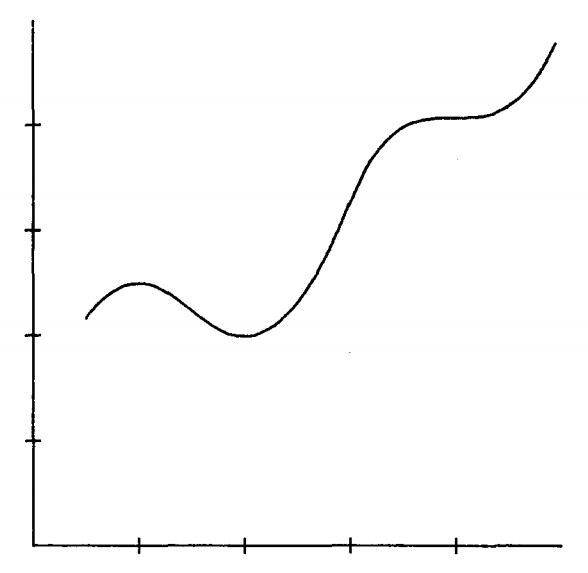
\includegraphics[scale=0.5]{img/pr. 477 1..png}

\task

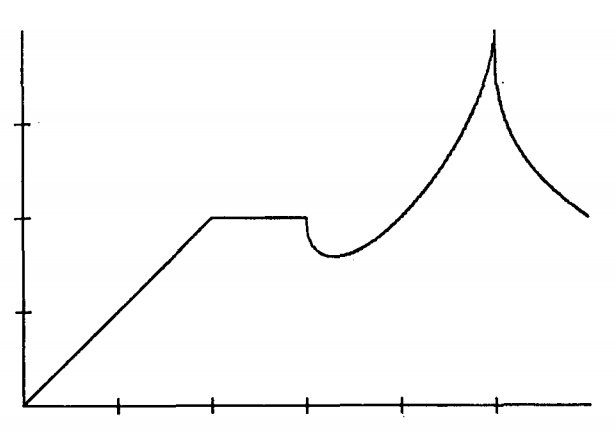
\includegraphics[scale=0.5]{img/pr. 477 2..png}

\end{tasks}
\end{defproblem}

\begin{defproblem}{diferencialny-pocet-478}
Načrtnite graf funkcie $f$ v okolí bodu $a$, ak
\begin{tasks}
\task $a=3,f(3)=1,f'(3)=f''(3)=f'''(3)=0,f^{(4)}<0$
\task $a=-1,f(-1)=-2,f'(-1)=1,f''(-1)=0,f'''(-1)>0$
\end{tasks}
\end{defproblem}
